% 第 11 章 广义 Stokes 定理
\chapter{广义 Stokes 定理}

广义版本的 Stokes 定理（此后我们简称为 Stokes 定理）是数学中一个异常强大而实用的工具. 我们在第 9.5 节已经遇到过它，在那里我们找到了一种把线积分基本定理、Stokes 定理的向量微积分版本和散度定理统一写成 $\int_M d\alpha=\int_{\partial M}\alpha$ 的常见方式. 更精确地说，Stokes 定理可以陈述如下.

\begin{theorem}[广义 Stokes 定理]\label{thm:11-1}
设 $M$ 是光滑的有向 $n$ 维流形，设 $\alpha$ 是 $M$ 上的 $(n-1)$-形式. 则
\[
\int_M d\alpha=\int_{\partial M}\alpha,
\]
其中 $\partial M$ 具有诱导定向.
\end{theorem}

它的证明几乎出现在微分几何的所有标准教材中，并且以各种不同的抽象程度和严格程度给出. 与本书的许多内容一样，我们将力求在可理解性、严格性和抽象性之间取得平衡. 特别是，我们给出的证明适用于"良好"的流形 $M$. 希望在学完本章之后，你能对整体图景有足够的理解，从而能够跟上一个数学上更严格的证明版本.

证明所遵循的一般策略是：先对一个非常具体而直接的简单情形证明定理，然后利用这个简单情形去证明越来越难的情形. 本质上，我们以"自举"（bootstrap）的方式一路推进到一般版本. 本章的每一节（最后一节除外）本质上都是"自举"步骤之一. 理解这些一般思想并不困难，但要得到一个完全严格、滴水不漏的证明，有时会让人觉得是在做琐碎、平凡而吹毛求疵的练习. 本章的最后一节利用第 5 章发展的可视化技术，在三维情形下把 Stokes 定理所要表达的内容可视化出来（至少在这些可视化技术适用的范围内）.

最后，Stokes 定理的证明要么基于 $k$ 维单位立方体（这正是我们将要采用的路线），要么有时基于 $k$ 维单纯形（simplex），通常简称为 $k$-单纯形（$k$-simplex）. （这是一个罕见的在用法上存在两种复数形式的英语单词，所以有时你也会看到 simplexes 这个词.）Stokes 定理在同调与上同调中的应用使得采用 $k$-单纯形是有用的. 虽然在单位 $k$-立方体与 $k$-单纯形之间可以相互转换，但这会给自举过程增加一层几乎令人不胜其烦的繁琐工作，所以我们不在此处做这一步. 实际上，这一步对理解整体图景几乎没有任何帮助，不过在阅读 Stokes 定理的其他证明时，你应该意识到这一点并保持留意.

\section{单位立方体 $I^k$}

我们首先需要讨论的是 $\mathbb{R}^n$（其中 $n\geq k$）中单位 $k$-立方体的定向. 单位 $k$-立方体一般记为 $I^k$. 在考察了 $k$-立方体 $I^k$ 的定向之后，我们将接着考察 $I^k$ 的\newterm{boundary}{边界}{boundary}以及边界块的定向. 一旦我们牢固地掌握了这一点，就可以对单位 $k$-立方体 $I^k$ 的情形证明 Stokes 定理.

\textbf{0 立方体 $I^0$}. 首先我们考虑 0-立方体. 0-立方体实际上并不怎么有趣，它只是一个点. 为方便起见，我们把立方体放在原点处. 因此，我们可以把 $\mathbb{R}^n$ 中的 0-立方体简单地看作一个点，记为 $\{0\}$. 由于是退化对象，0-立方体不像其他 $k$-立方体那样具有定向，不过我们将会看到，如有必要，我们可以给它赋予正定向或负定向.

\textbf{1 立方体 $I^1$}. 接下来我们考察单位 1-立方体 $I^1=\{x_1\in\mathbb{R}\mid 0\leq x_1\leq 1\}$，如图~\ref{fig:11-1} 所示. 我们说 $I^1\subset\mathbb{R}^1$ 的定向由体积形式 $dx_1$ 决定. 这是如何起作用的呢？考虑基于原点、指向 1-立方体方向的单位向量 $[1]$. 我们有 $dx_1([1])=1$，它是正的，所以这给出 $I^1$ 上的正定向. 相反的方向 $-[1]$ 给出 $dx_1(-[1])=-1$，这显然给出负定向，见图~\ref{fig:11-2}.

\begin{figure}[htbp]
  \centering
  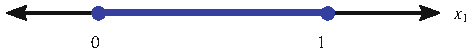
\includegraphics[width=0.561\linewidth]{images/vector/fig-11-1.pdf}
  \caption{画在 $x_1$-轴上的一维单位立方体.}
  \label{fig:11-1}
\end{figure}

\begin{figure}[htbp]
  \centering
  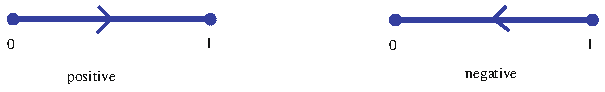
\includegraphics[width=0.728\linewidth]{images/vector/fig-11-2.pdf}
  \caption{一维单位立方体的两种定向. 定向由一维体积形式 $dx_1$ 决定，一般分别称为正定向（左）和负定向（右）.}
  \label{fig:11-2}
\end{figure}

\textbf{2 立方体 $I^2$}. 现在让我们考虑 2-立方体 $I^2=\{(x_1,x_2)\mid 0\leq x_i\leq 1,\ i=1,2\}$. 同样，体积形式 $dx_1\wedge dx_2$ 决定（我们常说诱导）$I^2$ 上的一个定向. 考虑两个单位向量
\[
e_1=\binom{1}{0},\qquad e_2=\binom{0}{1}.
\]
2-立方体正是由这两个单位向量张成的平行六面体，如图~\ref{fig:11-3} 所示. 利用二维体积形式 $dx_1\wedge dx_2$，我们有
\begin{align*}
dx_1\wedge dx_2\left(\binom{1}{0},\binom{0}{1}\right)=\begin{vmatrix}1&0\\0&1\end{vmatrix}=1>0, \\
dx_1\wedge dx_2\left(\binom{0}{1},\binom{1}{0}\right)=\begin{vmatrix}0&1\\1&0\end{vmatrix}=-1<0.
\end{align*}
因此，单位向量的次序决定了 2-立方体的定向. 次序
\[
\left\{\binom{1}{0},\binom{0}{1}\right\}
\]
表示正定向，而次序
\[
\left\{\binom{0}{1},\binom{1}{0}\right\}
\]
表示负定向. 正定向通常如图~\ref{fig:11-4} 所示用图形表示，而负定向通常如图~\ref{fig:11-5} 所示用图形表示.

\begin{figure}[htbp]
  \centering
  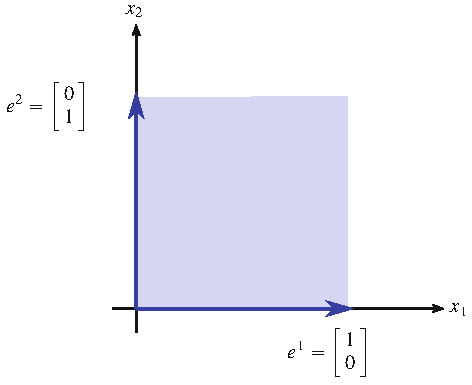
\includegraphics[width=0.559\linewidth]{images/vector/fig-11-3.pdf}
  \caption{二维单位立方体是由单位向量 $e_1$ 和 $e_2$ 张成的平行六面体.}
  \label{fig:11-3}
\end{figure}

\begin{figure}[htbp]
  \centering
  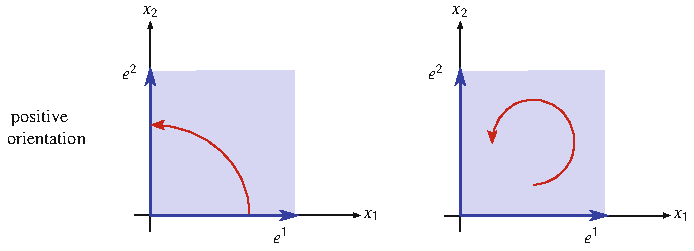
\includegraphics[width=0.822\linewidth]{images/vector/fig-11-4.pdf}
  \caption{利用体积形式 $dx_1\wedge dx_2$ 我们看到，次序 $\{e_1,e_2\}$，即先 $e_1$ 后 $e_2$，给出正定向. 图中展示了表示正定向的两种方式}
  \label{fig:11-4}
\end{figure}

\begin{figure}[htbp]
  \centering
  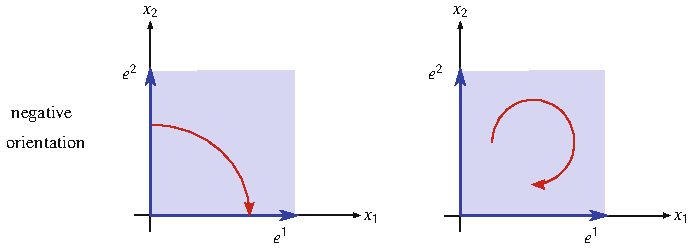
\includegraphics[width=0.822\linewidth]{images/vector/fig-11-5.pdf}
  \caption{利用体积形式 $dx_1\wedge dx_2$ 我们看到，次序 $\{e_2,e_1\}$，即先 $e_2$ 后 $e_1$，给出负定向. 图中展示了表示负定向的两种方式}
  \label{fig:11-5}
\end{figure}

\textbf{3 立方体 $I^3$}. 现在我们来看一看 3-立方体 $I^3=\{(x_1,x_2,x_3)\mid 0\leq x_i\leq 1,\ i=1,2,3\}$，如图~\ref{fig:11-6} 所示. 3-立方体正是由向量
\[
e_1=\begin{bmatrix}1\\0\\0\end{bmatrix},\qquad e_2=\begin{bmatrix}0\\1\\0\end{bmatrix},\qquad e_3=\begin{bmatrix}0\\0\\1\end{bmatrix}
\]
张成的平行六面体. 体积形式 $dx_1\wedge dx_2\wedge dx_3$ 决定（或诱导）$I^3$ 上的一个定向. 显然有
\[
dx_1\wedge dx_2\wedge dx_3\left(\begin{bmatrix}1\\0\\0\end{bmatrix},\begin{bmatrix}0\\1\\0\end{bmatrix},\begin{bmatrix}0\\0\\1\end{bmatrix}\right)=\begin{vmatrix}1&0&0\\0&1&0\\0&0&1\end{vmatrix}=1>0.
\]
因此，向量次序
\[
\left\{\begin{bmatrix}1\\0\\0\end{bmatrix},\begin{bmatrix}0\\1\\0\end{bmatrix},\begin{bmatrix}0\\0\\1\end{bmatrix}\right\}=\{e_1,e_2,e_3\}
\]
被认为是一个正定向. 正定向通常如图~\ref{fig:11-7} 所示用图形表示. 这正是所谓的"右手法则". 但注意，我们也有 $dx_1\wedge dx_2\wedge dx_3(e_2,e_3,e_1)=1$，所以 $\{e_2,e_3,e_1\}$ 也是一个正定向. 类似地，$dx_1\wedge dx_2\wedge dx_3(e_3,e_1,e_2)=1$，所以 $\{e_3,e_1,e_2\}$ 是又一个正定向. 于是我们看到，共有三种不同的次序给出 $I^3$ 的正定向. 接下来注意 $dx_1\wedge dx_2\wedge dx_3(e_2,e_1,e_3)=-1<0$，所以 $\{e_2,e_1,e_3\}$ 给出一个负定向，你可以把它看作"左手法则". 见图~\ref{fig:11-8}.

\begin{figure}[htbp]
  \centering
  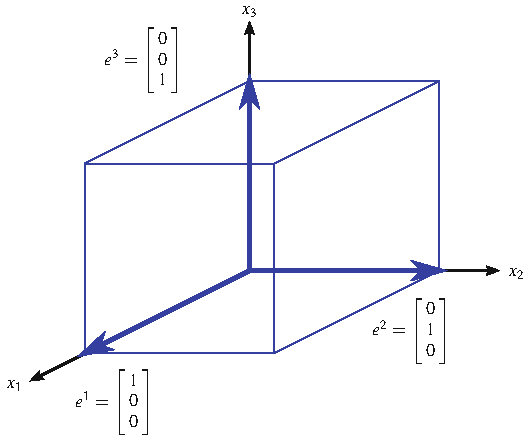
\includegraphics[width=0.628\linewidth]{images/vector/fig-11-6.pdf}
  \caption{三维单位立方体是由三个单位向量 $e_1$、$e_2$ 和 $e_3$ 张成的平行六面体}
  \label{fig:11-6}
\end{figure}

\begin{figure}[htbp]
  \centering
  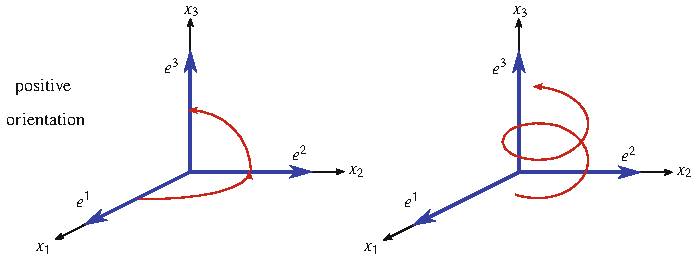
\includegraphics[width=0.827\linewidth]{images/vector/fig-11-7.pdf}
  \caption{利用体积形式 $dx_1\wedge dx_2\wedge dx_3$ 我们看到，次序 $\{e_1,e_2,e_3\}$，即先 $e_1$、再 $e_2$、再 $e_3$，给出正定向. 图中展示了表示正定向的两种方式. 三维中的正定向一般称为"右手法则"}
  \label{fig:11-7}
\end{figure}

\begin{figure}[htbp]
  \centering
  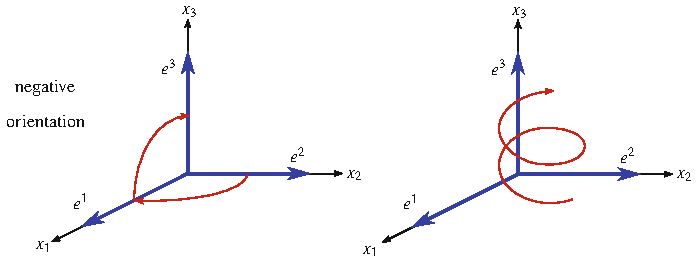
\includegraphics[width=0.827\linewidth]{images/vector/fig-11-8.pdf}
  \caption{利用体积形式 $dx_1\wedge dx_2\wedge dx_3$ 我们看到，次序 $\{e_2,e_1,e_3\}$，即先 $e_2$、再 $e_1$、再 $e_3$，给出负定向. 图中展示了表示负定向的两种方式. 三维中的负定向一般称为"左手法则"}
  \label{fig:11-8}
\end{figure}

\begin{question}\label{q:11-1}
给出 $I^3$ 负定向的三种次序是什么？
\end{question}

所以我们看到，给我们的基元素选取一个次序并不是标记或确定 $k$-立方体定向的一种很有效的方式. 这就是我们使用标准体积形式 $dx_1\wedge dx_2\wedge dx_3$——即下标按数值顺序排列的体积形式——的原因. 当然，这实际上归根结底还是为我们向量空间的基元素选取一个次序，但我们总得有个起点. 标准体积形式在每个单位立方体上诱导正定向和负定向，具体取决于我们如何排列用来生成立方体的单位向量.

\textbf{k 立方体 $I^k$}. 对于 $k>3$ 的 $I^k$，无论是 $k$-立方体还是其定向都无法画出，但思想是足够直观的. $k$-立方体是由单位向量 $e_1,e_2,\ldots,e_k$ 张成的平行六面体. 给定一个体积形式 $dx_1\wedge dx_2\wedge\cdots\wedge dx_k$，该体积形式就诱导一个定向. 例如，给定体积形式 $dx_1\wedge dx_2\wedge dx_3\wedge dx_4$，$e_1,e_2,e_3,e_4$ 的任何导致体积为正的次序都称为 $I^4$ 的正定向，任何导致体积为负的次序都称为负定向. 我们在图~\ref{fig:11-9} 中尝试"画出"$I^4$ 的一个正定向和一个负定向.

\begin{figure}[htbp]
  \centering
  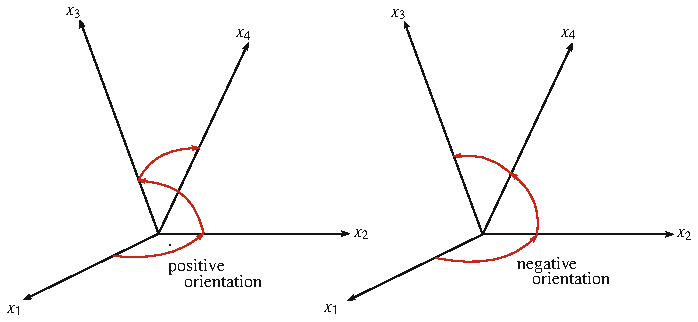
\includegraphics[width=0.827\linewidth]{images/vector/fig-11-9.pdf}
  \caption{为四维空间画出正定向（左）和负定向（右）的尝试. 由于有四个轴，它们不再能被画成彼此都与其他三个垂直，但应当理解为所画出的每个轴实际上都与其余三个垂直}
  \label{fig:11-9}
\end{figure}

\begin{question}\label{q:11-2}
求出 $e_1,e_2,e_3,e_4$ 的所有正定向和负定向.
\end{question}

\textbf{k-立方体的边界，$\partial I^k$}. 既然我们对单位立方体的定向有了一些概念，我们想要弄清楚单位立方体的边界是什么. 当然，你对边界是什么有一些直观的想法，但我们的目标是使这些想法在数学上精确. 我们还将考虑边界定向的思想，它起初可能有点令人困惑.

由于 0-立方体只是一个点，它没有边界. 我们起初并不考虑孤立点 $I^0$ 的定向，但在 $I^1$ 的边界这一背景下，我们将给一个点赋予定向. 首先我们将给出 $k$-立方体边界的一般定义，然后看一些边界的具体例子.

给定一个 $k$-立方体
\[
I^k=\left\{(x_1,\ldots,x_k)\,\bigl|\,0\leq x_i\leq 1,\ i=1,\ldots,k\right\},
\]
我们通过令 $x_i=0$ 来定义 $(i,0)$-面，于是有
\[
I^k_{(i,0)}=\left\{(x_1,\ldots,x_{i-1},0,x_{i+1},\ldots,x_k)\,\bigl|\,(x_1,\ldots,x_{i-1},0,x_{i+1},\ldots,x_k)\in I^k\right\},
\]
并通过令 $x_i=1$ 来定义 $(i,1)$-面，于是有
\[
I^k_{(i,1)}=\left\{(x_1,\ldots,x_{i-1},1,x_{i+1},\ldots,x_k)\,\bigl|\,(x_1,\ldots,x_{i-1},1,x_{i+1},\ldots,x_k)\in I^k\right\}.
\]
每个面 $I^k_{(i,a)}$（其中 $a=0,1$）将被赋予由 $(-1)^{i+a}$ 决定的定向. 若 $(-1)^{i+a}=1$，则定向为正；若 $(-1)^{i+a}=-1$，则定向为负. 我们将通过例子看出，为什么这是定义面的定向的恰当方式. $I^k$ 的边界记为 $\partial I^k$，它是 $I^k$ 的所有面连同所确定的定向的集合. 抽象地，我们写
\[
\partial I^k=\sum_{i=1}^{k}\sum_{a=0}^{1}(-1)^{i+a}I^k_{(i,a)},
\]
不过请记住，我们当然不是在通常意义下把这些面相加. 这仅仅是我们表示构成 $I^k$ 边界的各个面连同其各自定向的集合的方式.

\textbf{求 $\partial I^1$}. 让我们看看这对 $I^1$ 是如何进行的. 我们有
\[
I^1_{(1,0)}=\{(0)\},\qquad I^1_{(1,1)}=\{(1)\}.
\]
接下来我们看到，$I^1_{(1,0)}$ 具有负定向，因为 $(-1)^{1+0}=-1$；而 $I^1_{(1,1)}$ 具有正定向，因为 $(-1)^{1+1}=1$. 这在图~\ref{fig:11-10} 中作了说明. 最后，我们这样表示 $I^1$ 的边界：
\[
\partial I^1=\sum_{i=1}^{1}\sum_{a=0}^{1}(-1)^{i+a}I^1_{(i,a)}=I^1_{(1,1)}-I^1_{(1,0)}.
\]

\begin{figure}[htbp]
  \centering
  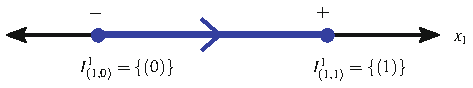
\includegraphics[width=0.561\linewidth]{images/vector/fig-11-10.pdf}
  \caption{带正定向的 1-立方体 $I^1$，连同带负定向的面 $I^1_{(1,0)}$ 和带正定向的面 $I^1_{(1,1)}$}
  \label{fig:11-10}
\end{figure}

\textbf{求 $\partial I^2$}. 接下来我们把注意力转向 $I^2$. 2-立方体有四个面，由下式给出：
\begin{align*}
I^2_{(1,0)}=\{(0,x_2)\mid(0,x_2)\in I^2\},\qquad
I^2_{(1,1)}=\{(1,x_2)\mid(1,x_2)\in I^2\}, \\
I^2_{(2,0)}=\{(x_1,0)\mid(x_1,0)\in I^2\},\qquad
I^2_{(2,1)}=\{(x_1,1)\mid(x_1,1)\in I^2\}.
\end{align*}
带边界的 2-立方体的图画如图~\ref{fig:11-11} 所示. 我们现在给 2-立方体的面赋予如下定向：
\begin{align*}
I^2_{(1,0)}\ \text{的定向由 }(-1)^{1+0}=-1\ \text{决定}\Rightarrow\text{负}, \\
I^2_{(1,1)}\ \text{的定向由 }(-1)^{1+1}=1\ \text{决定}\Rightarrow\text{正}, \\
I^2_{(2,0)}\ \text{的定向由 }(-1)^{2+0}=1\ \text{决定}\Rightarrow\text{正}, \\
I^2_{(2,1)}\ \text{的定向由 }(-1)^{2+1}=-1\ \text{决定}\Rightarrow\text{负},
\end{align*}
于是我们得到带定向边界的 2-立方体的图画，如图~\ref{fig:11-12} 所示. 注意，通过给面 $I^2_{(i,a)}$ 赋予由 $(-1)^{i+a}$ 决定的定向，我们的边界定向在某种意义上是自洽的，它们以一致的方式"绕"2-立方体一周. 我们这样表示 2-立方体的边界：
\[
\partial I^2=\sum_{i=1}^{2}\sum_{a=0}^{1}(-1)^{i+a}I^2_{(i,a)}=-I^2_{(1,0)}+I^2_{(1,1)}+I^2_{(2,0)}-I^2_{(2,1)}.
\]

\begin{figure}[htbp]
  \centering
  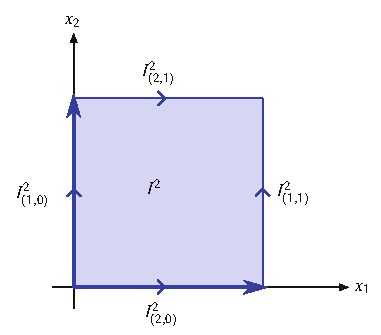
\includegraphics[width=0.549\linewidth]{images/vector/fig-11-11.pdf}
  \caption{2-立方体 $I^2$ 连同其边界，边界由四个面 $I^2_{(1,0)}$、$I^2_{(1,1)}$、$I^2_{(2,0)}$ 和 $I^2_{(2,1)}$ 给出. 四个面都以正定向显示}
  \label{fig:11-11}
\end{figure}

\begin{figure}[htbp]
  \centering
  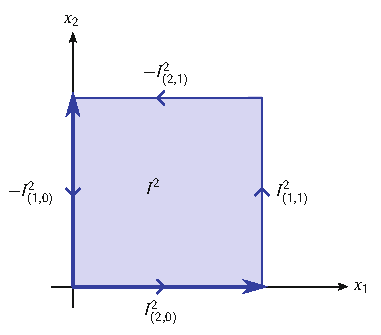
\includegraphics[width=0.549\linewidth]{images/vector/fig-11-12.pdf}
  \caption{2-立方体 $I^2$ 连同其四个边界面，此处以由公式确定的定向显示. 例如，面 $I^2_{(i,a)}$ 的定向由 $(-1)^{i+a}$ 是正还是负来决定}
  \label{fig:11-12}
\end{figure}

\begin{question}\label{q:11-3}
图~\ref{fig:11-11} 中的 2-立方体是这样画的：四个边界都用箭头显示为正定向. 解释为什么箭头是它们所示的方向.
\end{question}

\textbf{求 $\partial\partial I^1$}. 退后一步，我们可以看出 $\partial\partial I^1=0$ 也成立. 我们已有 $\partial I^1=\{(1)\}-\{(0)\}$，其中 $(0)$ 和 $(1)$ 是 $\mathbb{R}^1$ 上的点. 由于点没有边界，我们说 $\partial\{(0)\}=0$，$\partial\{(1)\}=0$，于是得到
\[
\partial\partial I^1=\partial\{(1)\}-\partial\{(0)\}=0-0=0.
\]

\textbf{求 $\partial\partial I^2$}. 现在，我们将更进一步，求出边界元素的边界. 也就是说，我们将求 $\partial\bigl(-I^2_{(1,0)}\bigr)$、$\partial I^2_{(1,1)}$、$\partial I^2_{(2,0)}$ 和 $\partial\bigl(-I^2_{(2,1)}\bigr)$. 我们从 $\partial I^2_{(2,0)}$ 开始. 我们看到
\begin{align*}
\bigl(I^2_{(2,0)}\bigr)^1_{(1,0)}=\{(0,0)\}\quad\text{具有定向 }(-1)^{1+0}=-1\Rightarrow\text{负}, \\
\bigl(I^2_{(2,0)}\bigr)^1_{(1,1)}=\{(1,0)\}\quad\text{具有定向 }(-1)^{1+1}=1\Rightarrow\text{正}.
\end{align*}
我们在图~\ref{fig:11-13} 中展示了 $\partial I^2_{(2,0)}$.

\begin{figure}[htbp]
  \centering
  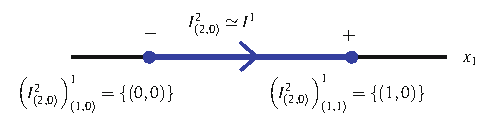
\includegraphics[width=0.720\linewidth]{images/vector/fig-11-13.pdf}
  \caption{$I^2_{(2,0)}$ 的边界由带负定向的 $\bigl(I^2_{(2,0)}\bigr)^1_{(1,0)}$ 和带正定向的 $\bigl(I^2_{(2,0)}\bigr)^1_{(1,1)}$ 给出}
  \label{fig:11-13}
\end{figure}

为了求 $\partial I^2_{(1,1)}$，我们需要特别注意下标. 回顾
\[
I^2_{(1,1)}=\left\{\bigl(1,x_2\bigr)\,\bigl|\,\bigl(1,x_2\bigr)\in I^2\right\}.
\]
注意，$I^2_{(1,1)}$ 现在实际上是一个 1-立方体，即 $I^2_{(1,1)}\simeq I^1$. 所以当我们想取这个 1-立方体的 $(1,0)$ 边界时，这个 1 所指的变量是这个 1-立方体中的第一个变量，而它实际上仍被标记为 $x_2$，
\[
\partial\bigl(I^2_{(1,1)}\bigr)^1_{(1,0)}=\{(1,0)\}.
\]
类似地，
\[
\partial\bigl(I^2_{(1,1)}\bigr)^1_{(1,1)}=\{(1,1)\}.
\]
至于定向，
\begin{align*}
\bigl(I^2_{(1,1)}\bigr)^1_{(1,0)}=\{(1,0)\}\quad\text{具有定向 }(-1)^{1+0}=-1\Rightarrow\text{负}, \\
\bigl(I^2_{(1,1)}\bigr)^1_{(1,1)}=\{(1,1)\}\quad\text{具有定向 }(-1)^{1+1}=1\Rightarrow\text{正}.
\end{align*}
然后我们可以像图~\ref{fig:11-14} 那样画出 $\partial I^2_{(1,1)}$.

\begin{figure}[htbp]
  \centering
  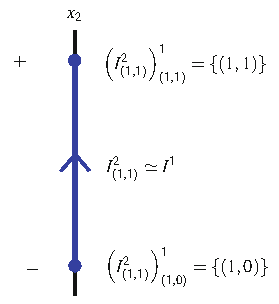
\includegraphics[width=0.402\linewidth]{images/vector/fig-11-14.pdf}
  \caption{$I^2_{(1,1)}$ 的边界由带负定向的 $\bigl(I^2_{(1,1)}\bigr)^1_{(1,0)}$ 和带正定向的 $\bigl(I^2_{(1,1)}\bigr)^1_{(1,1)}$ 给出}
  \label{fig:11-14}
\end{figure}

现在对于 $\partial\bigl(-I^2_{(2,1)}\bigr)$，我们看到
\begin{align*}
\bigl(-I^2_{(2,1)}\bigr)^1_{(1,0)}=\{(0,1)\}\quad\text{具有定向 }-(-1)^{1+0}=1\Rightarrow\text{正}, \\
\bigl(-I^2_{(2,1)}\bigr)^1_{(1,1)}=\{(1,1)\}\quad\text{具有定向 }-(-1)^{1+1}=-1\Rightarrow\text{负},
\end{align*}
从而允许我们像图~\ref{fig:11-15} 那样画出 $\partial\bigl(-I^2_{(2,1)}\bigr)$.

\begin{figure}[htbp]
  \centering
  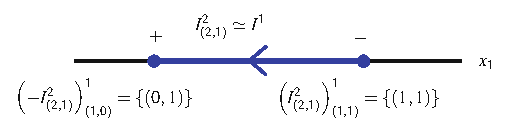
\includegraphics[width=0.729\linewidth]{images/vector/fig-11-15.pdf}
  \caption{$-I^2_{(2,1)}$ 的边界由带正定向的 $\bigl(-I^2_{(2,1)}\bigr)^1_{(1,0)}$ 和带负定向的 $\bigl(-I^2_{(2,1)}\bigr)^1_{(1,1)}$ 给出}
  \label{fig:11-15}
\end{figure}

最后，对于 $\partial\bigl(-I^2_{(1,0)}\bigr)$，我们看到
\begin{align*}
\bigl(-I^2_{(1,0)}\bigr)^1_{(1,0)}=\{(0,0)\}\quad\text{具有定向 }-(-1)^{1+0}=1\Rightarrow\text{正}, \\
\bigl(-I^2_{(1,0)}\bigr)^1_{(1,1)}=\{(0,1)\}\quad\text{具有定向 }-(-1)^{1+1}=-1\Rightarrow\text{负},
\end{align*}
从而允许我们像图~\ref{fig:11-16} 那样画出 $\partial\bigl(-I^2_{(1,0)}\bigr)$.

\begin{figure}[htbp]
  \centering
  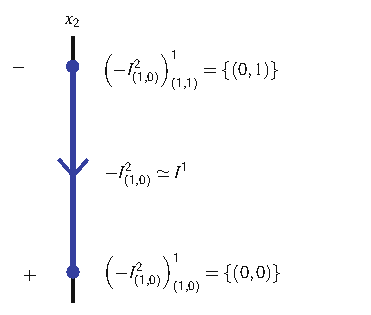
\includegraphics[width=0.534\linewidth]{images/vector/fig-11-16.pdf}
  \caption{$-I^2_{(1,0)}$ 的边界由带正定向的 $\bigl(-I^2_{(1,0)}\bigr)^1_{(1,0)}$ 和带负定向的 $\bigl(-I^2_{(1,0)}\bigr)^1_{(1,1)}$ 给出}
  \label{fig:11-16}
\end{figure}

把所有结果放在一起，对于 $\partial\partial I^2$，我们有图~\ref{fig:11-17} 中的图画，它给出
\[
\begin{aligned}
\partial\partial I^2&=\partial\bigl(-I^2_{(1,0)}\bigr)+\partial I^2_{(1,1)}+\partial I^2_{(2,0)}+\partial\bigl(-I^2_{(2,1)}\bigr)\\
&=\{(0,0)\}-\{(0,1)\}-\{(1,0)\}+\{(1,1)\}-\{(0,0)\}+\{(1,0)\}+\{(0,1)\}-\{(1,1)\}\\
&=0.
\end{aligned}
\]
于是我们看到，边界元素及其定向的定义方式使得边界的边界为零，这在直觉上说得通. 毕竟，闭曲线没有边界，而 2-立方体的边界正是一条闭曲线.

\begin{figure}[htbp]
  \centering
  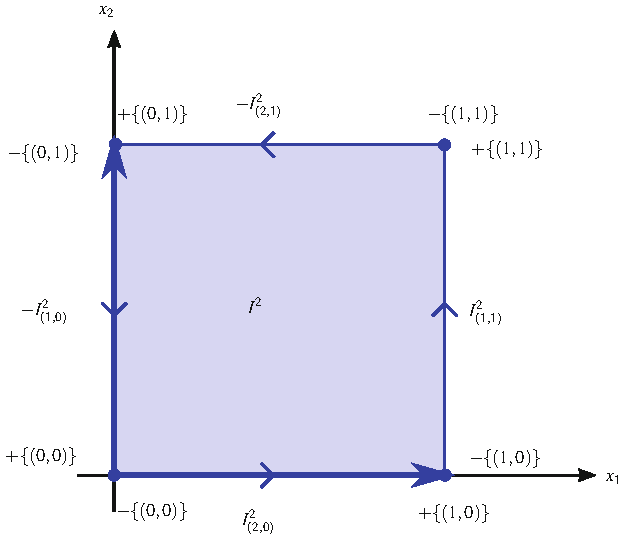
\includegraphics[width=0.742\linewidth]{images/vector/fig-11-17.pdf}
  \caption{为了得到 $\partial\partial I^2$ 的图画，我们把图~\ref{fig:11-13}、\ref{fig:11-14}、\ref{fig:11-15} 和 \ref{fig:11-16} 拼在一起}
  \label{fig:11-17}
\end{figure}

\textbf{求 $\partial I^3$}. 现在我们将考虑 $I^3$. 首先求 $I^3$ 的面，然后求这些面的定向，我们将用它们来求 $\partial I^3$. $I^3$ 显然有六个面，由下式给出：
\begin{align*}
I^3_{(1,0)}=\{(0,x_2,x_3)\mid 0\leq x_2,x_3\leq 1\}=\text{后面}, \\
I^3_{(1,1)}=\{(1,x_2,x_3)\mid 0\leq x_2,x_3\leq 1\}=\text{前面}, \\
I^3_{(2,0)}=\{(x_1,0,x_3)\mid 0\leq x_1,x_3\leq 1\}=\text{左面}, \\
I^3_{(2,1)}=\{(x_1,1,x_3)\mid 0\leq x_1,x_3\leq 1\}=\text{右面}, \\
I^3_{(3,0)}=\{(x_1,x_2,0)\mid 0\leq x_1,x_2\leq 1\}=\text{底面}, \\
I^3_{(3,1)}=\{(x_1,x_2,1)\mid 0\leq x_1,x_2\leq 1\}=\text{顶面},
\end{align*}
并在图~\ref{fig:11-18} 中作了展示.

\begin{figure}[htbp]
  \centering
  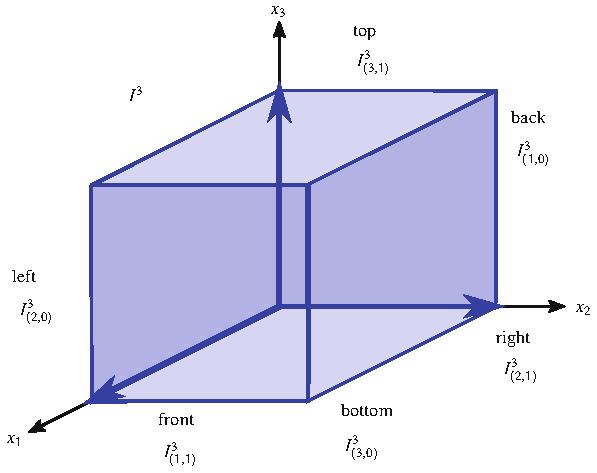
\includegraphics[width=0.859\linewidth]{images/vector/fig-11-18.pdf}
  \caption{3-立方体 $I^3$ 连同其六个面}
  \label{fig:11-18}
\end{figure}

我们首先展示 $I^3$ 全部六个面的正定向. 决定前面和后面定向的体积形式是 $dx_2\wedge dx_3$，因为前面和后面位于 $(x_2,x_3)$-平面中. 考虑两个向量
\[
\begin{bmatrix}0\\1\\0\end{bmatrix},\qquad\begin{bmatrix}0\\0\\1\end{bmatrix}
\]
在后面的点 $p=(0,0,0)$ 处和前面的点 $q=(1,0,0)$ 处. 对这两个点，我们都有
\begin{align*}
dx_2\wedge dx_3(p)\left(\begin{bmatrix}0\\1\\0\end{bmatrix}_{\!p},\begin{bmatrix}0\\0\\1\end{bmatrix}_{\!p}\right)=\begin{vmatrix}1&0\\0&1\end{vmatrix}=1, \\
dx_2\wedge dx_3(q)\left(\begin{bmatrix}0\\1\\0\end{bmatrix}_{\!q},\begin{bmatrix}0\\0\\1\end{bmatrix}_{\!q}\right)=\begin{vmatrix}1&0\\0&1\end{vmatrix}=1.
\end{align*}
前面和后面的正定向如图~\ref{fig:11-19} 所示.

\begin{figure}[htbp]
  \centering
  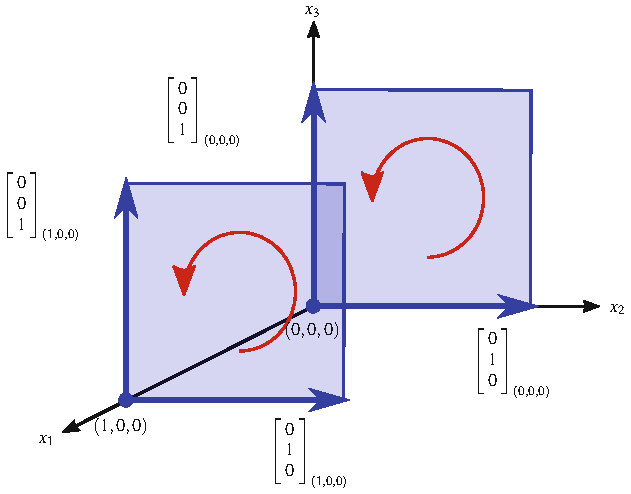
\includegraphics[width=0.748\linewidth]{images/vector/fig-11-19.pdf}
  \caption{带正定向显示的 $I^3$ 的前面和后面}
  \label{fig:11-19}
\end{figure}

决定左面和右面正定向的体积形式是 $dx_1\wedge dx_3$，因为左面和右面位于 $(x_1,x_3)$-平面中. 与前面完全一样，考虑两个向量
\[
\begin{bmatrix}1\\0\\0\end{bmatrix},\qquad\begin{bmatrix}0\\0\\1\end{bmatrix}
\]
在左面的点 $p=(0,0,0)$ 处和右面的点 $q=(0,1,0)$ 处. 对这两个点，我们都有
\begin{align*}
dx_1\wedge dx_3(p)\left(\begin{bmatrix}1\\0\\0\end{bmatrix}_{\!p},\begin{bmatrix}0\\0\\1\end{bmatrix}_{\!p}\right)=\begin{vmatrix}1&0\\0&1\end{vmatrix}=1, \\
dx_1\wedge dx_3(q)\left(\begin{bmatrix}1\\0\\0\end{bmatrix}_{\!q},\begin{bmatrix}0\\0\\1\end{bmatrix}_{\!q}\right)=\begin{vmatrix}1&0\\0&1\end{vmatrix}=1.
\end{align*}
左面和右面的正定向如图~\ref{fig:11-20} 所示.

\begin{figure}[htbp]
  \centering
  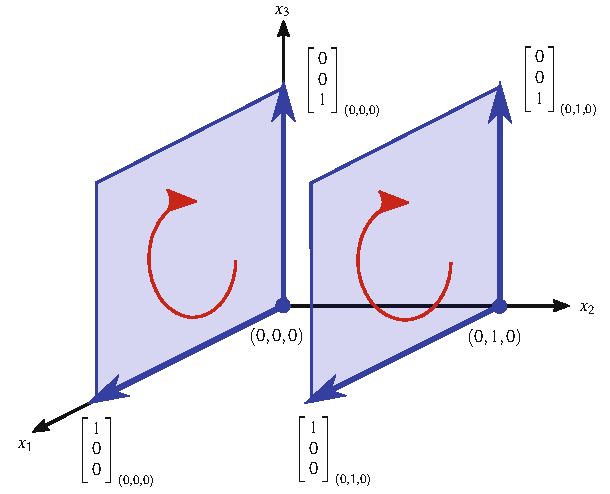
\includegraphics[width=0.724\linewidth]{images/vector/fig-11-20.pdf}
  \caption{带正定向显示的 $I^3$ 的左面和右面}
  \label{fig:11-20}
\end{figure}

\begin{question}\label{q:11-4}
对顶面和底面做同样的分析，以得到图~\ref{fig:11-21} 所示的这两个面的正定向.
\end{question}

\begin{figure}[htbp]
  \centering
  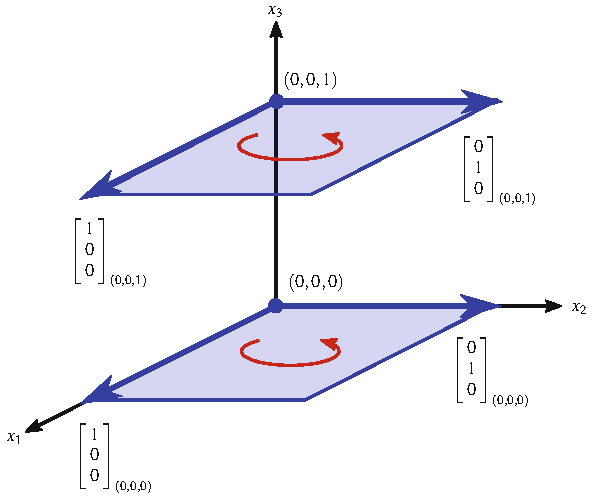
\includegraphics[width=0.703\linewidth]{images/vector/fig-11-21.pdf}
  \caption{带正定向显示的 $I^3$ 的顶面和底面}
  \label{fig:11-21}
\end{figure}

现在我们算出六个面的定向.
\begin{align*}
I^3_{(1,0)}\ \text{的定向由 }(-1)^{1+0}=-1\ \text{决定}\Rightarrow\text{负}, \\
I^3_{(1,1)}\ \text{的定向由 }(-1)^{1+1}=+1\ \text{决定}\Rightarrow\text{正}, \\
I^3_{(2,0)}\ \text{的定向由 }(-1)^{2+0}=+1\ \text{决定}\Rightarrow\text{正}, \\
I^3_{(2,1)}\ \text{的定向由 }(-1)^{2+1}=-1\ \text{决定}\Rightarrow\text{负}, \\
I^3_{(3,0)}\ \text{的定向由 }(-1)^{3+0}=-1\ \text{决定}\Rightarrow\text{负}, \\
I^3_{(3,1)}\ \text{的定向由 }(-1)^{3+1}=+1\ \text{决定}\Rightarrow\text{正}.
\end{align*}
把所有结果放在一起，我们可以写出 $I^3$ 的边界：
\[
\partial I^3=\sum_{i=1}^{3}\sum_{a=0}^{1}(-1)^{i+a}I^3_{(i,a)}
=-I^3_{(1,0)}+I^3_{(1,1)}+I^3_{(2,0)}-I^3_{(2,1)}-I^3_{(3,0)}+I^3_{(3,1)}.
\]

\begin{question}\label{q:11-5}
画出单位立方体 $I^3$ 的草图，包括各个面的适当定向. 这些定向看起来是否彼此吻合？
\end{question}

\textbf{求 $\partial\partial I^3$}. 现在我们想求 $\partial I^3$ 的边界. 回顾，$\partial I^3$ 由六个不同的 2-立方体组成. 我们将从求底面 $I^3_{(3,0)}$ 的边开始：
\begin{align*}
\bigl(I^3_{(3,0)}\bigr)^2_{(1,0)}=\{(0,x_2,0)\mid 0\leq x_2\leq 1\}\quad\text{具有定向 }(-1)^{3+0}(-1)^{1+0}=1, \\
\bigl(I^3_{(3,0)}\bigr)^2_{(1,1)}=\{(1,x_2,0)\mid 0\leq x_2\leq 1\}\quad\text{具有定向 }(-1)^{3+0}(-1)^{1+1}=-1, \\
\bigl(I^3_{(3,0)}\bigr)^2_{(2,0)}=\{(x_1,0,0)\mid 0\leq x_1\leq 1\}\quad\text{具有定向 }(-1)^{3+0}(-1)^{2+0}=-1, \\
\bigl(I^3_{(3,0)}\bigr)^2_{(2,1)}=\{(x_1,1,0)\mid 0\leq x_1\leq 1\}\quad\text{具有定向 }(-1)^{3+0}(-1)^{2+1}=1.
\end{align*}
类似地，顶面 $I^3_{(3,1)}$ 的边为
\begin{align*}
\bigl(I^3_{(3,1)}\bigr)^2_{(1,0)}=\{(0,x_2,1)\mid 0\leq x_2\leq 1\}\quad\text{具有定向 }(-1)^{3+1}(-1)^{1+0}=-1, \\
\bigl(I^3_{(3,1)}\bigr)^2_{(1,1)}=\{(1,x_2,1)\mid 0\leq x_2\leq 1\}\quad\text{具有定向 }(-1)^{3+1}(-1)^{1+1}=1, \\
\bigl(I^3_{(3,1)}\bigr)^2_{(2,0)}=\{(x_1,0,1)\mid 0\leq x_1\leq 1\}\quad\text{具有定向 }(-1)^{3+1}(-1)^{2+0}=1, \\
\bigl(I^3_{(3,1)}\bigr)^2_{(2,1)}=\{(x_1,1,1)\mid 0\leq x_1\leq 1\}\quad\text{具有定向 }(-1)^{3+1}(-1)^{2+1}=-1.
\end{align*}
我们在图~\ref{fig:11-22} 中展示了 $I^3$ 的底面和顶面连同其边界边的定向.

\begin{figure}[htbp]
  \centering
  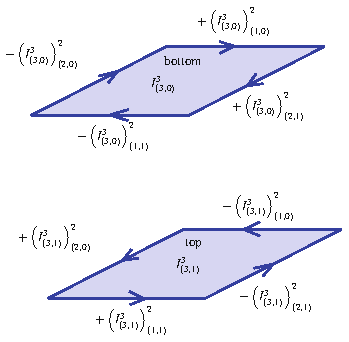
\includegraphics[width=0.650\linewidth]{images/vector/fig-11-22.pdf}
  \caption{3-立方体的底面和顶面，连同其边界的定向}
  \label{fig:11-22}
\end{figure}

确保你理解上面的记号是如何工作的. 底面/顶面的情形是最简单的情形. 对于后面/前面和左面/右面，记号中有一些有点棘手的地方. 让我们首先考虑后面 $I^3_{(1,0)}=\{(0,x_2,x_3)\mid 0\leq x_2,x_3\leq 1\}$，它是一个 2-立方体. 让我们首先考虑 $\bigl(I^3_{(1,0)}\bigr)^2_{(1,0)}$. 对于 3-立方体，变量是 $(x_1,x_2,x_3)$. $I^3_{(1,0)}$ 中的 $(1,0)$ 表示第一个变量 $x_1$ 被替换为 $0$. 但现在让我们考虑 3-立方体的后面，它是一个 2-立方体，即 $\bigl(I^3_{(1,0)}\bigr)^2_{(1,0)}$. 对于这个 2-立方体，变量是 $(x_2,x_3)$，所以 $\bigl(I^3_{(1,0)}\bigr)^2_{(1,0)}$ 中第二个 $(1,0)$ 表示第一个变量被替换为 $0$，但在这种情况下第一个变量是 $x_2$. 于是我们有
\[
\bigl(I^3_{(1,0)}\bigr)^2_{(1,0)}=\{(0,0,x_3)\mid 0\leq x_3\leq 1\}.
\]
其定向为 $(-1)^{1+0}(-1)^{1+0}=1$，是正的. 类似地，我们有
\begin{align*}
\bigl(I^3_{(1,0)}\bigr)^2_{(1,1)}=\{(0,1,x_3)\mid 0\leq x_3\leq 1\}\quad\text{具有定向 }(-1)^{1+0}(-1)^{1+1}=-1\Rightarrow\text{负}, \\
\bigl(I^3_{(1,0)}\bigr)^2_{(2,0)}=\{(0,x_2,0)\mid 0\leq x_2\leq 1\}\quad\text{具有定向 }(-1)^{1+0}(-1)^{2+0}=-1\Rightarrow\text{负}, \\
\bigl(I^3_{(1,0)}\bigr)^2_{(2,1)}=\{(0,x_2,1)\mid 0\leq x_2\leq 1\}\quad\text{具有定向 }(-1)^{1+0}(-1)^{2+1}=1\Rightarrow\text{正}.
\end{align*}
3-立方体的后面连同边界定向如图~\ref{fig:11-23} 所示.

\begin{figure}[htbp]
  \centering
  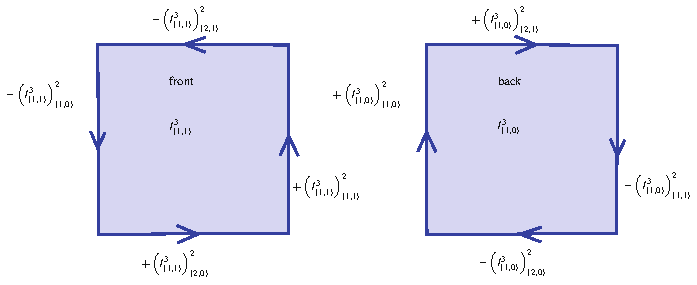
\includegraphics[width=0.960\linewidth]{images/vector/fig-11-23.pdf}
  \caption{3-立方体 $I^3$ 的前面和后面，连同其边界的定向}
  \label{fig:11-23}
\end{figure}

\begin{question}\label{q:11-6}
求前面 $I^3_{(1,1)}=\{(1,x_2,x_3)\mid 0\leq x_2,x_3\leq 1\}$ 的四条边界边，并求这些边的定向. 你的答案应与图~\ref{fig:11-23} 一致.
\end{question}

\begin{question}\label{q:11-7}
证明：当考虑定向时，$\bigl(I^3_{(3,1)}\bigr)^2_{(1,0)}=-\bigl(I^3_{(1,0)}\bigr)^2_{(2,1)}$，且 $\bigl(I^3_{(3,0)}\bigr)^2_{(1,0)}=-\bigl(I^3_{(1,0)}\bigr)^2_{(2,0)}$. 见图~\ref{fig:11-24}.
\end{question}

\begin{figure}[htbp]
  \centering
  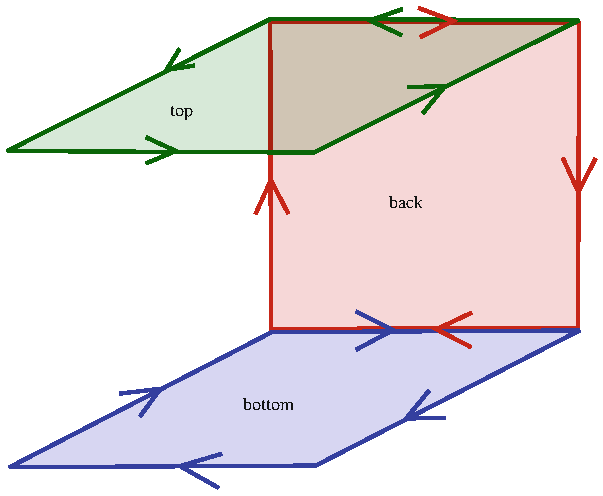
\includegraphics[width=0.715\linewidth]{images/vector/fig-11-24.pdf}
  \caption{3-立方体 $I^3$ 的顶面、底面和后面，连同其边界. 注意三个面的边界在何处相同：当考虑定向时，我们有 $\bigl(I^3_{(3,1)}\bigr)^2_{(1,0)}=-\bigl(I^3_{(1,0)}\bigr)^2_{(2,1)}$，且 $\bigl(I^3_{(3,0)}\bigr)^2_{(1,0)}=-\bigl(I^3_{(1,0)}\bigr)^2_{(2,0)}$}
  \label{fig:11-24}
\end{figure}

\begin{question}\label{q:11-8}
证明：当考虑定向时，$\bigl(I^3_{(3,1)}\bigr)^2_{(1,1)}=-\bigl(I^3_{(1,1)}\bigr)^2_{(2,1)}$，且 $\bigl(I^3_{(3,0)}\bigr)^2_{(1,1)}=-\bigl(I^3_{(1,1)}\bigr)^2_{(2,0)}$. 见图~\ref{fig:11-25}.
\end{question}

\begin{figure}[htbp]
  \centering
  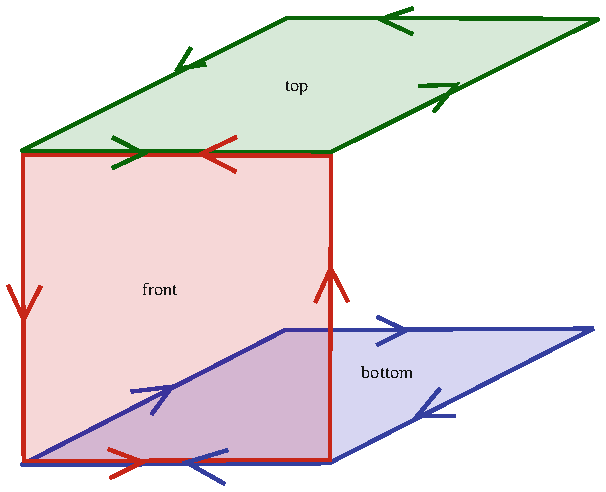
\includegraphics[width=0.719\linewidth]{images/vector/fig-11-25.pdf}
  \caption{3-立方体 $I^3$ 的顶面、底面和前面，连同其边界. 注意三个面的边界在何处相同：当考虑定向时，我们有 $\bigl(I^3_{(3,1)}\bigr)^2_{(1,1)}=-\bigl(I^3_{(1,1)}\bigr)^2_{(2,1)}$，且 $\bigl(I^3_{(3,0)}\bigr)^2_{(1,1)}=-\bigl(I^3_{(1,1)}\bigr)^2_{(2,0)}$}
  \label{fig:11-25}
\end{figure}

\begin{question}\label{q:11-9}
求左面 $I^3_{(2,0)}=\{(x_1,0,x_3)\mid 0\leq x_1,x_3\leq 1\}$ 和右面 $I^3_{(2,1)}=\{(x_1,1,x_3)\mid 0\leq x_1,x_3\leq 1\}$ 的四条边界边，并求这八条边界边的定向. 把顶面、左面和底面画在一起，然后再把顶面、右面和底面画在一起.
\end{question}

通过检查各种草图，你应该能够看出，下列 1-立方体是等同的：
\begin{align*}
\bigl(I^3_{(2,0)}\bigr)^2_{(1,0)}=\bigl(I^3_{(1,0)}\bigr)^2_{(1,0)}, \\
\bigl(I^3_{(2,1)}\bigr)^2_{(1,1)}=\bigl(I^3_{(1,1)}\bigr)^2_{(1,0)}, \\
\bigl(I^3_{(2,0)}\bigr)^2_{(2,0)}=\bigl(I^3_{(3,0)}\bigr)^2_{(2,0)}, \\
\bigl(I^3_{(2,0)}\bigr)^2_{(2,1)}=\bigl(I^3_{(3,1)}\bigr)^2_{(2,0)}.
\end{align*}

\begin{question}\label{q:11-10}
把所有结果放在一起，证明 $\partial\partial I^3=0$.
\end{question}

\textbf{求 $\partial\partial I^k$}. 考虑 $i\leq j\leq k-1$ 且 $a,b=0,1$ 的情形：
\[
\begin{aligned}
\bigl(I^k_{(i,a)}\bigr)^{k-1}_{(j,b)}&=\bigl\{(x_1,\ldots,x_{i-1},a,x_{i+1},\ldots,x_k)\bigr\}^{k-1}_{(j,b)}\\
&=\bigl\{(x_1,\ldots,x_{i-1},a,x_i,\ldots,x_{k-1})\bigr\}^{k-1}_{(j,b)}\quad(\text{重新标记为 }(k-1)\text{-立方体的变量名})\\
&=\bigl\{(x_1,\ldots,x_{i-1},a,x_i,\ldots,x_{j-1},b,x_{j+1},\ldots,x_{k-1})\bigr\}\\
&=\bigl\{(x_1,\ldots,x_{i-1},a,x_{i+1},\ldots,x_j,b,x_{j+2},\ldots,x_k)\bigr\}\\
&\qquad(\text{重新标记为 }k\text{-立方体的变量名}),
\end{aligned}
\]
所以当我们使用 $k$-立方体的变量名时，$b$ 位于第 $j+1$ 个位置. 我们还有
\[
\begin{aligned}
\bigl(I^k_{(j+1,b)}\bigr)^{k-1}_{(i,a)}&=\bigl\{(x_1,\ldots,x_j,b,x_{j+2},\ldots,x_k)\bigr\}^{k-1}_{(i,a)}\\
&=\bigl\{(x_1,\ldots,x_{i-1},a,x_{i+1},\ldots,x_j,b,x_{j+2},\ldots,x_k)\bigr\}\\
&\qquad(\text{由于 }i\leq j\text{，无需重新标记}).
\end{aligned}
\]
因此，对 $i\leq j\leq k-1$，我们有
\[
\bigl(I^k_{(i,a)}\bigr)^{k-1}_{(j,b)}=\bigl(I^k_{(j+1,b)}\bigr)^{k-1}_{(i,a)}.
\]

\begin{question}\label{q:11-11}
解释为什么条件 $i\leq j\leq k-1$ 并不构成限制. 也就是说，$\partial I^k$ 的每个边界元素都被包括了.
\end{question}

\begin{question}\label{q:11-12}
证明对一般的 $I^k$，有 $\partial\partial I^k=0$.
\end{question}

\section{基础情形：$I^k$ 上的 Stokes 定理}

在覆盖了所有这些必要的背景材料之后，Stokes 定理的实际证明其实并不那么困难. 正如我们前面所说，我们将以"自举"的方式一路推进到完全一般的情形. 第一步是在 $k$-立方体 $I^k$ 上证明 Stokes 定理. 给定定义在单位 $k$-立方体 $I^k$ 的某个邻域上的 $(k-1)$-形式 $\alpha$，我们想证明
\[
\int_{I^k}d\alpha=\int_{\partial I^k}\alpha.
\]

首先，$\alpha$ 是定义在 $I^k\subset\mathbb{R}^k$ 的某个邻域上的 $(k-1)$-形式，所以 $\alpha$ 具有一般形式
\[
\begin{aligned}
\alpha&=\alpha_1(x_1,\ldots,x_k)\,dx_2\wedge dx_3\wedge\cdots\wedge dx_k\\
&\quad+\alpha_2(x_1,\ldots,x_k)\,dx_1\wedge dx_3\wedge\cdots\wedge dx_k\\
&\quad+\cdots\\
&\quad+\alpha_k(x_1,\ldots,x_k)\,dx_1\wedge dx_2\wedge\cdots\wedge dx_{k-1}\\
&=\sum_{i=1}^{k}\alpha_i(x_1,\ldots,x_k)\,dx_1\wedge\cdots\wedge\widehat{dx_i}\wedge\cdots\wedge dx_k,
\end{aligned}
\]
其中 $\widehat{dx_i}$ 表示 $dx_i$ 被省略，$\alpha_i:\mathbb{R}^k\to\mathbb{R}$（$1\leq i\leq k$）是定义在 $I^k$ 的某个邻域上的实值函数. 我们知道外微分 $d$ 是线性的，这意味着
\[
d\left(\sum_{i=1}^{k}\alpha_i\,dx_1\wedge\cdots\wedge\widehat{dx_i}\wedge\cdots\wedge dx_k\right)=\sum_{i=1}^{k}d\left(\alpha_i\,dx_1\wedge\cdots\wedge\widehat{dx_i}\wedge\cdots\wedge dx_k\right).
\]
我们还知道积分是线性的，所以
\[
\int_{I^k}\sum_{i=1}^{k}d\left(\alpha_i\,dx_1\wedge\cdots\wedge\widehat{dx_i}\wedge\cdots\wedge dx_k\right)=\sum_{i=1}^{k}\int_{I^k}d\left(\alpha_i\,dx_1\wedge\cdots\wedge\widehat{dx_i}\wedge\cdots\wedge dx_k\right).
\]

现在让我们考虑 $(k-1)$-形式 $\alpha$ 的第一项，即 $\alpha_1\,dx_2\wedge\cdots\wedge dx_k$. 于是我们有
\[
\begin{aligned}
\int_{I^k}d\bigl(\alpha_1\,dx_2\wedge\cdots\wedge dx_k\bigr)
&=\int_{I^k}\frac{\partial\alpha_1}{\partial x_1}\,dx_1\wedge dx_2\wedge\cdots\wedge dx_k\\
&=\int_{x_k=0}^{1}\cdots\int_{x_2=0}^{1}\int_{x_1=0}^{1}\frac{\partial\alpha_1}{\partial x_1}\,dx_1dx_2\cdots dx_k\\
&\quad(\text{传统积分（定向无关紧要）})\\
&=\int_{x_k=0}^{1}\cdots\int_{x_2=0}^{1}\Bigl[\alpha_1(x_1,x_2,\ldots,x_k)\Bigr]_{0}^{1}\,dx_2\cdots dx_k\\
&\quad(\text{微积分基本定理})\\
&=\int_{x_k=0}^{1}\cdots\int_{x_2=0}^{1}\Bigl(\alpha_1(1,x_2,\ldots,x_k)\\
&\quad-\alpha_1(0,x_2,\ldots,x_k)\Bigr)\,dx_2\cdots dx_k\\
&=\int_{x_k=0}^{1}\cdots\int_{x_2=0}^{1}\alpha_1(1,x_2,\ldots,x_k)\\
&\quad\cdot dx_2\cdots dx_k\\
&\quad(\text{$\alpha_1$ 限制在面 }I^k_{(1,1)}\text{ 上的积分})\\
&\quad-\int_{x_k=0}^{1}\cdots\int_{x_2=0}^{1}\alpha_1(0,x_2,\ldots,x_k)\\
&\quad\cdot dx_2\cdots dx_k\\
&\quad(\text{$\alpha_1$ 限制在面 }I^k_{(1,0)}\text{ 上的积分})\\
&=\int_{I^k_{(1,1)}}\alpha_1\,dx_2\wedge\cdots\wedge dx_k\\
&\qquad-\int_{I^k_{(1,0)}}\alpha_1\,dx_2\wedge\cdots\wedge dx_k.
\end{aligned}
\]

正如你所注意到的，我们把记号从第二行中的 $dx_1\wedge dx_2\wedge\cdots\wedge dx_k$ 换成第三行中的 $dx_1dx_2\cdots dx_k$，然后再从传统记号换回最后一行中的 $dx_2\wedge\cdots\wedge dx_k$. 正如你大概还记得的（来自前面某章），你在微积分课上学到的传统积分与微分形式的积分只在一个方面有所不同：它不追踪曲面的定向. 我们做这种切换是为了使用微积分基本定理，而我们只知道基本定理的传统记号形式. 在使用传统记号的过程中，我们所做的一切都不会影响我们正在其上积分的立方体的定向. 我们之所以认识到这一点，是因为当我们从形式记号切换到传统记号、然后再从传统记号切换回形式记号时，次序是一致的. 要看到这一点，请比较第二行中的体积形式 $dx_1\wedge dx_2\wedge\cdots\wedge dx_k$ 与最后一行中的体积形式 $dx_2\wedge\cdots\wedge dx_k$. 最后一行中的体积形式比第一行中的低一维，它缺少 $dx_1$ 项，因为我们针对 $dx_1$ 项进行了积分；但除了这一处省略之外，其余 $k-1$ 项的次序没有改变. 因为当我们要换回形式记号时剩余项的次序没有改变，所以一切都是一致的. 为方便起见，我们将改写刚得到的这个等式，把 $\alpha$ 的第一项记为 $\alpha_1$ 而不是 $\alpha_1\,dx_2\wedge\cdots\wedge dx_k$，于是我们有
\[
\int_{I^k}d\alpha_1=\int_{I^k_{(1,1)}}\alpha_1-\int_{I^k_{(1,0)}}\alpha_1.
\]
这诚然是对记号的轻微滥用，但它确实大大简化了事情.

现在我们花一点时间来说明，$(k-1)$-形式 $\alpha_1\,dx_2\wedge\cdots\wedge dx_k$ 在 $\partial I^k$ 的所有其他面上的积分为零，并且我们在 $I^k$ 的边界上积分 $\alpha_1$ 时所预期得到的唯一贡献，正是上述等式右端所给出的那个贡献. $\partial I^k$ 的所有其他面都具有 $I^k_{(i,a)}$ 的形式，其中 $2\leq i\leq k$，$a=0,1$.

现在回顾 $dx_2\wedge dx_3\wedge\cdots\wedge dx_k$ 的作用：它把平行六面体投影到 $(x_2\cdots x_k)$-平面并求该投影的体积. 我们有兴趣在 $I^k$ 的各个面上取 $\alpha_1$ 的积分. 考虑 $I^k_{(1,1)}$，它是一个 $(k-1)$ 维平行六面体. 把 $I^k_{(1,1)}$ 投影到 $(x_2\cdots x_k)$-平面并求这个投影的体积，得到的体积为 1. 类似地，把 $I^k_{(1,0)}$ 投影到 $(x_2\cdots x_k)$-平面，得到的体积也为 1. 见图~\ref{fig:11-26}. 于是我们能够在这个面上取 $\alpha_1$ 的积分.

\begin{figure}[htbp]
  \centering
  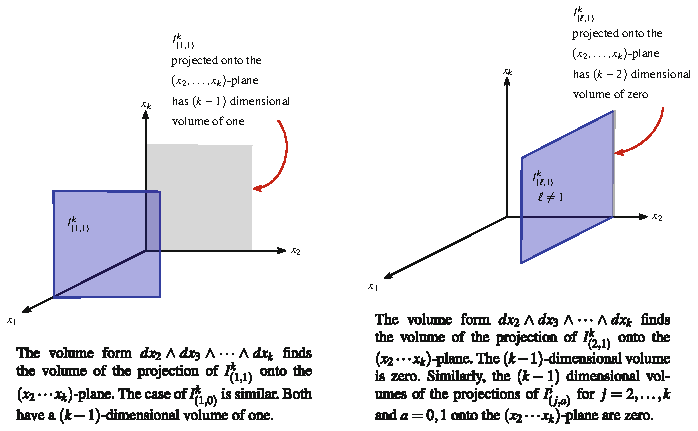
\includegraphics[width=0.960\linewidth]{images/vector/fig-11-26.pdf}
  \caption{求 $I^k$ 的各面投影到 $(x_2\cdots x_k)$-平面时的体积}
  \label{fig:11-26}
\end{figure}

但现在考虑 $I^k_{(2,1)}$. 当把这个面投影到 $(x_2\cdots x_k)$-平面上时，其 $(k-1)$ 维体积为零，因为 $I^k_{(2,1)}$ 在 $(x_2\cdots x_k)$-平面上的投影是一个 $(k-2)$ 维集合，它具有零 $(k-1)$ 维体积. 因此 $\int_{I^k_{(2,1)}}\alpha_1=0$. 类似地，我们得出对所有 $j=2,\ldots,k$ 和 $a=0,1$，$\int_{I^k_{(j,a)}}\alpha_1=0$，见图~\ref{fig:11-26}. 于是，$I^k$ 的边界上唯一能给出非零贡献的积分，就是我们已有的 $\int_{I^k_{(1,1)}}\alpha_1$ 和 $\int_{I^k_{(1,0)}}\alpha_1$.

另外，注意我们所发现的：
\[
\int_{I^k}d\alpha_1=\int_{I^k_{(1,1)}}\alpha_1-\int_{I^k_{(1,0)}}\alpha_1.
\]
在 $I^k_{(1,1)}$ 上的积分是正的，这正与面 $I^k_{(1,1)}$ 在 $I^k$ 的边界中的定向一致，因为 $(-1)^{1+1}=1$. 类似地，在 $I^k_{(1,0)}$ 上的积分是负的，这正与面 $I^k_{(1,0)}$ 在 $I^k$ 的边界中的定向一致，因为 $(-1)^{1+0}=-1$. 于是我们可以——事实上也确实——作如下定义
\[
\int_{I^k_{(1,1)}}\alpha_1-\int_{I^k_{(1,0)}}\alpha_1\equiv\int_{I^k_{(1,1)}-I^k_{(1,0)}}\alpha_1,
\]
这允许我们写
\[
\int_{I^k}d\alpha_1=\int_{I^k_{(1,1)}-I^k_{(1,0)}}\alpha_1.
\]

现在我们将考察 $\alpha$ 的第二项. 我们有
\[
\begin{aligned}
\int_{I^k}d\bigl(\alpha_2\,dx_1\wedge dx_3\wedge\cdots\wedge dx_k\bigr)
&=\int_{I^k}\frac{\partial\alpha_2}{\partial x_2}\,dx_2\wedge dx_1\wedge dx_3\wedge\cdots\wedge dx_k\\
&=(-1)\int_{I^k}\frac{\partial\alpha_2}{\partial x_2}\,dx_1\wedge dx_2\wedge dx_3\wedge\cdots\wedge dx_k\\
&=(-1)\int_{x_k=0}^{1}\cdots\int_{x_2=0}^{1}\int_{x_1=0}^{1}\frac{\partial\alpha_2}{\partial x_2}\,dx_1dx_2\cdots dx_k\\
&\quad(\text{传统积分（定向无关紧要）})\\
&=(-1)\int_{x_k=0}^{1}\cdots\int_{x_1=0}^{1}\int_{x_2=0}^{1}\frac{\partial\alpha_2}{\partial x_2}\,dx_2dx_1\cdots dx_k\\
&\quad(\text{Fubini 定理})\\
&=(-1)\int_{x_k=0}^{1}\cdots\int_{x_1=0}^{1}\Bigl[\alpha_2(x_1,x_2,x_3,\ldots,x_k)\Bigr]_{0}^{1}\\
&\quad\cdot dx_1dx_3\cdots dx_k\\
&\quad(\text{微积分基本定理})\\
&=(-1)\int_{x_k=0}^{1}\cdots\int_{x_3=0}^{1}\int_{x_1=0}^{1}\\
&\quad\Bigl(\alpha_2(x_1,1,x_3,\ldots,x_k)\\
&\quad-\alpha_2(x_1,0,x_3,\ldots,x_k)\Bigr)\,dx_1dx_3\cdots dx_k\\
&=(-1)\int_{x_k=0}^{1}\cdots\int_{x_3=0}^{1}\int_{x_1=0}^{1}\alpha_2(x_1,1,x_3,\ldots,x_k)\\
&\quad\cdot dx_1dx_3\cdots dx_k\\
&\quad(\text{$\alpha_2$ 限制在面 }I^k_{(2,1)}\text{ 上的积分})\\
&\quad-(-1)\int_{x_k=0}^{1}\cdots\int_{x_3=0}^{1}\int_{x_1=0}^{1}\alpha_2(x_1,0,x_3,\ldots,x_k)\\
&\quad\cdot dx_1dx_3\cdots dx_k\\
&\quad(\text{$\alpha_2$ 限制在面 }I^k_{(2,0)}\text{ 上的积分})\\
&=-\int_{I^k_{(2,1)}}\alpha_2\,dx_1\wedge dx_3\wedge\cdots\wedge dx_k\\
&\quad+\int_{I^k_{(2,0)}}\alpha_2\,dx_1\wedge dx_3\wedge\cdots\wedge dx_k\\
&=\int_{-I^k_{(2,1)}+I^k_{(2,0)}}\alpha_2\\
&\quad\cdot dx_1\wedge dx_3\wedge\cdots\wedge dx_k.
\end{aligned}
\]

正如你所注意到的，我们把记号从第三行中的 $dx_1\wedge dx_2\wedge\cdots\wedge dx_k$ 换成第四行中的 $dx_1dx_2\cdots dx_k$，然后再换回倒数第二行中的 $dx_1\wedge dx_3\wedge\cdots\wedge dx_k$. 我们做这种切换是为了同时使用 Fubini 定理和微积分基本定理，而我们只知道这两个定理的传统记号形式. 你可能会想，在应用 Fubini 定理时交换积分次序会不会改变我们的体积-定向，但由于传统积分不追踪体积-定向的符号，这种改变不会改变相伴的体积-定向符号. 这意味着重要的是，当我们在传统记号与形式记号之间来回切换时，体积形式的定向是一致的. 例如，第三行中的体积形式是 $dx_1\wedge dx_2\wedge dx_3\wedge\cdots\wedge dx_k$，而倒数第二行中的体积形式是 $dx_1\wedge dx_3\wedge\cdots\wedge dx_k$. 虽然倒数第二行中缺少 $dx_2$（因为我们针对该项进行了积分），但剩余项的次序没有改变，因此是一致的.

注意这些符号再次与 $I^k$ 的边界中各面的定向相符. 这使我们能够改写这个计算的结果. 如果我们另外采用我们之前使用过的同样的记号滥用，把 $\alpha_2\,dx_1\wedge dx_3\wedge\cdots\wedge dx_k$ 写成 $\alpha_2$，我们就得到等式
\[
\int_{I^k}d\alpha_2=\int_{-I^k_{(2,1)}+I^k_{(2,0)}}\alpha_2.
\]

既然我们已经对 $(k-1)$-形式的头两项做了这个处理，你就对我们将要如何进行有了些概念. 现在我们将对整个
\[
\alpha=\sum_{i=1}^{k}\alpha_i\,dx_1\wedge\cdots\wedge\widehat{dx_i}\wedge\cdots\wedge dx_k
\]
做这个处理，其中 $\widehat{dx_i}$ 表示第 $i$ 项 $dx_i$ 被省略. 首先我们求 $d\alpha$，
\[
\begin{aligned}
d\left(\sum_{i=1}^{k}\alpha_i\,dx_1\wedge\cdots\wedge\widehat{dx_i}\wedge\cdots\wedge dx_k\right)
&=\sum_{i=1}^{k}d\left(\alpha_i\,dx_1\wedge\cdots\wedge\widehat{dx_i}\wedge\cdots\wedge dx_k\right)\\
&=\sum_{i=1}^{k}\frac{\partial\alpha_i}{\partial x_i}\,dx_i\wedge dx_1\wedge\cdots\wedge\widehat{dx_i}\wedge\cdots\wedge dx_k\\
&=\sum_{i=1}^{k}(-1)^{i-1}\frac{\partial\alpha_i}{\partial x_i}\,dx_1\wedge\cdots\wedge dx_i\wedge\cdots\wedge dx_k,
\end{aligned}
\]
其中进行 $i-1$ 次对换给出符号 $(-1)^{i-1}$，也就是
\[
d\alpha=\sum_{i=1}^{k}(-1)^{i-1}\frac{\partial\alpha_i}{\partial x_i}\,dx_1\wedge\cdots\wedge dx_i\wedge\cdots\wedge dx_k.
\]

现在我们已经有了 $d\alpha$，接下来进行积分：
\[
\begin{aligned}
\int_{I^k}d\alpha
&=\int_{I^k}\left(\sum_{i=1}^{k}(-1)^{i-1}\frac{\partial\alpha_i}{\partial x_i}\,dx_1\wedge\cdots\wedge dx_k\right)\\
&=\sum_{i=1}^{k}(-1)^{i-1}\int_{I^k}\frac{\partial\alpha_i}{\partial x_i}\,dx_1\wedge\cdots\wedge dx_k\\
&=\sum_{i=1}^{k}(-1)^{i-1}\int_{0}^{1}\cdots\int_{0}^{1}\frac{\partial\alpha_i}{\partial x_i}\,dx_i\,dx_1\cdots\widehat{dx_i}\cdots dx_k\quad(\text{传统积分（定向无关紧要）})\\
&=\sum_{i=1}^{k}(-1)^{i-1}\int_{0}^{1}\cdots\int_{0}^{1}\Bigl[\alpha_i(x_1,\ldots,x_k)\Bigr]_{0}^{1}\,dx_1\cdots\widehat{dx_i}\cdots dx_k\quad(\text{微积分基本定理})\\
&=\sum_{i=1}^{k}(-1)^{i-1}\int_{0}^{1}\cdots\int_{0}^{1}\Bigl(\alpha_i(x_1,\ldots,1,\ldots,x_k)\\
&\quad-\alpha_i(x_1,\ldots,0,\ldots,x_k)\Bigr)\,dx_1\cdots\widehat{dx_i}\cdots dx_k\\
&=\sum_{i=1}^{k}(-1)^{i-1}\left(\int_{I^k_{(i,1)}}\alpha_i\,dx_1\wedge\cdots\wedge\widehat{dx_i}\wedge\cdots\wedge dx_k\right.\\
&\quad\left.-\int_{I^k_{(i,0)}}\alpha_i\,dx_1\wedge\cdots\wedge\widehat{dx_i}\wedge\cdots\wedge dx_k\right)\\
&=\sum_{i=1}^{k}\left[(-1)^{i-1}\int_{I^k_{(i,1)}}\alpha_i\,dx_1\wedge\cdots\wedge\widehat{dx_i}\wedge\cdots\wedge dx_k\right.\\
&\quad\left.+(-1)^{i}\int_{I^k_{(i,0)}}\alpha_i\,dx_1\wedge\cdots\wedge\widehat{dx_i}\wedge\cdots\wedge dx_k\right].
\end{aligned}
\]

在最后一行中，我们利用了如下事实：$I^k_{(i,1)}$ 在 $\partial I^k$ 中的定向为 $(-1)^{i+1}$，而 $(-1)^{i-1}=(-1)^{i+1}$，所以积分前的符号与 $I^k_{(i,1)}$ 在 $\partial I^k$ 中的定向相符；$I^k_{(i,0)}$ 在 $\partial I^k$ 中的定向为 $(-1)^{i+0}$，而 $(-1)^{i+0}=(-1)^{i}$，所以积分前的符号与 $I^k_{(i,0)}$ 在 $\partial I^k$ 中的定向相符. 此外，$\alpha$ 的 $\alpha_i$ 项只对面 $I^k_{(i,1)}$ 和 $I^k_{(i,0)}$ 有贡献，因此我们可以把这些项加在一起. 于是
\[
\begin{aligned}
\int_{I^k}d\alpha
&=\sum_{i=1}^{k}\left[\int_{(-1)^{i-1}I^k_{(i,1)}}\alpha_i\,dx_1\wedge\cdots\wedge\widehat{dx_i}\wedge\cdots\wedge dx_k\right.\\
&\quad\left.+\int_{(-1)^{i}I^k_{(i,0)}}\alpha_i\,dx_1\wedge\cdots\wedge\widehat{dx_i}\wedge\cdots\wedge dx_k\right]\\
&=\sum_{i=1}^{k}\int_{(-1)^{i-1}I^k_{(i,1)}+(-1)^{i}I^k_{(i,0)}}\alpha_i\,dx_1\wedge\cdots\wedge\widehat{dx_i}\wedge\cdots\wedge dx_k\\
&=\int_{\sum_{i=1}^{k}\left[(-1)^{i-1}I^k_{(i,1)}+(-1)^{i}I^k_{(i,0)}\right]}\\
&\quad\sum_{i=1}^{k}\alpha_i\,dx_1\wedge\cdots\wedge\widehat{dx_i}\wedge\cdots\wedge dx_k\\
&=\int_{\partial I^k}\alpha.
\end{aligned}
\]

于是，对于定义在单位 $k$-立方体某个邻域上的 $(k-1)$-形式 $\alpha$，我们已经证明了
\[
\int_{I^k}d\alpha=\int_{\partial I^k}\alpha.
\]
这正是单位 $k$-立方体情形下的 Stokes 定理. 既然我们有了这个至关重要的基础情形，其余情形就相当快速而容易地随之而来.

\section{由 $I^k$ 参数化的流形}

现在假设我们有一个带边流形 $M$，它由单位立方体参数化. 也就是说，我们有一个映射 $\varphi:\mathbb{R}^k\to\mathbb{R}^n$，其中 $\varphi(I^k)=M$. 见图~\ref{fig:11-27}. 实际上，$\varphi$ 甚至不必是一一的. 映射 $\varphi$ 通常称为 $M$ 上的\newterm{singular-k-cube}{奇异 $k$-立方体}{singular $k$-cube}. "奇异"一词表明映射 $\varphi$ 不必是一一的. 要求 $\varphi$ 非奇异是更严格的条件，也没有必要，不过我们将要求 $\varphi$ 可微.

\begin{figure}[htbp]
  \centering
  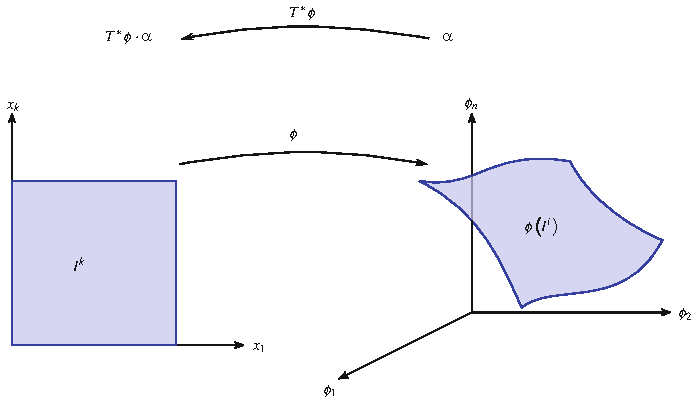
\includegraphics[width=0.835\linewidth]{images/vector/fig-11-27.pdf}
  \caption{映射 $\varphi:\mathbb{R}^k\to\mathbb{R}^n$，其中 $\varphi(I^k)=M$. 定义在 $\varphi(I^k)$ 上的微分形式 $\alpha$ 可以通过 $T^*\varphi$ 拉回到定义在 $I^k$ 上的微分形式 $T^*\varphi\cdot\alpha$}
  \label{fig:11-27}
\end{figure}

在阅读其他书中 Stokes 定理的证明时，请记住 $T^*\varphi$ 是我们对 $\varphi^*$ 的一个略微非标准的记号. 在这一点上我们不会过于严格，但我们也要求 $\varphi$ 尊重边界，我们的意思是：若 $M=\varphi(I^k)$，则 $\partial M=\varphi(\partial I^k)$. 换言之，我们要求
\[
\partial\varphi(I^k)=\varphi(\partial I^k).
\]
这是足够一般且"显然"的，不会引起问题. 我们还需要回顾关于拉回形式积分的如下恒等式：对某个区域 $R$，
\[
\int_{\varphi(R)}\alpha=\int_{R}T^*\varphi\cdot\alpha.
\]
在上一章中，我们会把它写成带 $\varphi^{-1}(R)$ 的形式，但如果 $\varphi$ 是奇异的，即不是一一的，那么 $\varphi$ 就不可逆，所以我们在此避免这种记号. 最后，回顾外微分与拉回可交换，即
\[
d\circ T^*\varphi=T^*\varphi\circ d,
\]
在大多数微分几何教材中写作 $d\circ\varphi^*=\varphi^*\circ d$.

利用这一切，最后一步几乎平淡无奇：
\[
\begin{aligned}
\int_M d\alpha&=\int_{\varphi(I^k)}d\alpha\quad(\text{记号})\\
&=\int_{I^k}T^*\varphi\cdot d\alpha\quad(\text{拉回形式的积分})\\
&=\int_{I^k}d\bigl(T^*\varphi\cdot\alpha\bigr)\quad(\text{外微分与拉回可交换})\\
&=\int_{\partial I^k}T^*\varphi\cdot\alpha\quad(\text{基础情形})\\
&=\int_{\varphi(\partial I^k)}\alpha\quad(\text{拉回形式的积分})\\
&=\int_{\partial\varphi(I^k)}\alpha\quad(\text{$\varphi$ 尊重边界})\\
&=\int_{\partial M}\alpha\quad(\text{记号}).
\end{aligned}
\]
于是，对 $M$ 上的奇异 $k$-立方体，我们有
\[
\int_M d\alpha=\int_{\partial M}\alpha.
\]

\section{链上的 Stokes 定理}

现在假设我们的带边流形 $M$ 不能由一个映射 $\varphi$ 很好地参数化，但可以被分解为长方体区域，其中每一个都可由一个映射 $\varphi_i:I^k\to\varphi_i(I^k)$（$i=1,\ldots,r$）参数化. 我们将假设有限个映射 $\varphi_i$ 就足够了. 见图~\ref{fig:11-28}. 但有一个警告：这里我们对记号 $\varphi_i$ 的使用与以往各章不同. 这里每个 $\varphi_i$ 都是一个映射 $\varphi_i:\mathbb{R}^k\to\mathbb{R}^n$，而以前我们有一个映射 $\varphi:\mathbb{R}^k\to\mathbb{R}^n$，定义为 $\varphi=(\varphi_1,\varphi_2,\ldots,\varphi_k)$，其中每个 $\varphi_i$ 是实值函数 $\varphi_i:\mathbb{R}^k\to\mathbb{R}$.

\begin{figure}[htbp]
  \centering
  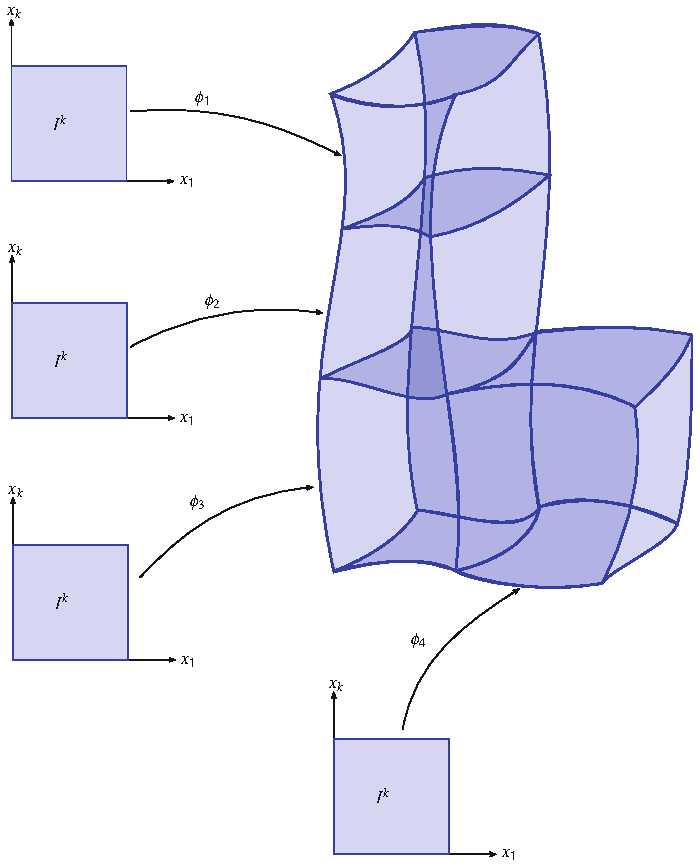
\includegraphics[width=0.840\linewidth]{images/vector/fig-11-28.pdf}
  \caption{流形 $M$ 可以被分解为有限个长方体区域，其中每一个都由映射 $\varphi_i:I^k\to\varphi_i(I^k)\subset M$ 参数化. 若 $\varphi_i(I^k)$ 的内部互不重叠、$\varphi_i(I^k)$ 的边界彼此吻合，且 $M=\bigcup_{i=1}^{r}\varphi_i(I^k)$，则 $\varphi_1+\varphi_2+\cdots+\varphi_r$ 称为 $M$ 上的奇异 $k$-链}
  \label{fig:11-28}
\end{figure}

我们这样选取用来参数化流形 $M$ 的映射，使得 $\varphi_i(I^k)$ 的内部互不重叠，并且 $\varphi_i(I^k)$ 的边界彼此吻合. 我们不会深入过多的技术细节，相信上面的图画能给你正确的直观想法. $M$ 上的一个\newterm{singular-k-chain}{奇异 $k$-链}{singular $k$-chain} $C$ 定义为
\[
C=\varphi_1+\varphi_2+\cdots+\varphi_r,
\]
其中每个 $\varphi_i$（$i=1,\ldots,r$）都是 $M$ 上的奇异 $k$-立方体. 换言之，我们有
\[
M=\bigcup_{i=1}^{r}\varphi_i(I^k)\equiv\varphi_1(I^k)+\varphi_2(I^k)+\cdots+\varphi_r(I^k)\equiv C(I^k).
\]

我们还将假设奇异 $k$-链 $C$ 的所有内部边界都彼此吻合，并具有相反的定向，如图~\ref{fig:11-29} 所示. $\varphi_i\bigl(I^k_{(l,1)}\bigr)$ 的定向是 $(-1)^{l+1}$，而 $\varphi_j\bigl(I^k_{(l,0)}\bigr)$ 的定向是 $(-1)^{l+0}$，所以 $\alpha$ 在 $\varphi_i\bigl(I^k_{(l,1)}\bigr)$ 上的积分贡献被 $\alpha$ 在 $\varphi_j\bigl(I^k_{(l,0)}\bigr)$ 上的积分贡献所抵消. 我们有
\[
\begin{aligned}
\partial(M)&=\partial\bigl(C(I^k)\bigr)\\
&=\partial\bigl(\varphi_1(I^k)+\varphi_2(I^k)+\cdots+\varphi_r(I^k)\bigr)\\
&=\partial\bigl(\varphi_1(I^k)\bigr)+\partial\bigl(\varphi_2(I^k)\bigr)+\cdots+\partial\bigl(\varphi_r(I^k)\bigr)\\
&=\varphi_1\bigl(\partial(I^k)\bigr)+\varphi_2\bigl(\partial(I^k)\bigr)+\cdots+\varphi_r\bigl(\partial(I^k)\bigr).
\end{aligned}
\]

\begin{figure}[htbp]
  \centering
  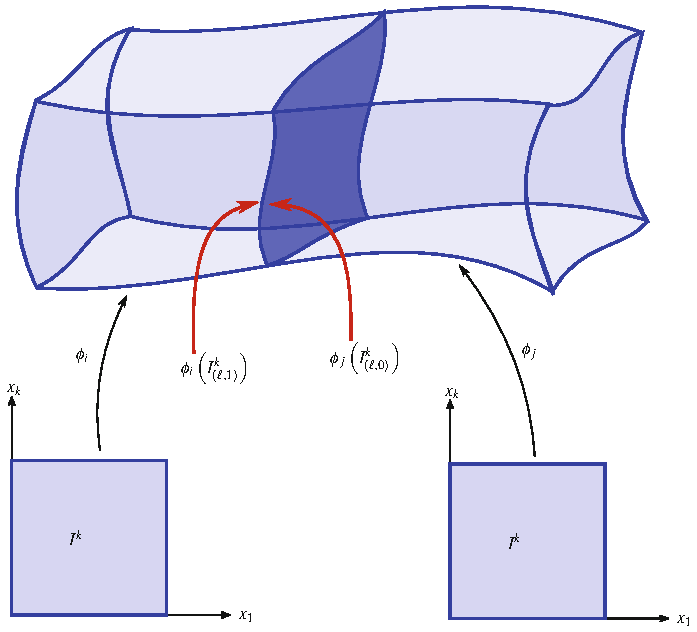
\includegraphics[width=0.960\linewidth]{images/vector/fig-11-29.pdf}
  \caption{这里两个长方体区域的边界彼此吻合且具有相反的定向. 即 $\varphi_i\bigl(I^k_{(l,1)}\bigr)=-\varphi_j\bigl(I^k_{(l,0)}\bigr)$}
  \label{fig:11-29}
\end{figure}

所以在链上证明 Stokes 定理是容易的：
\[
\begin{aligned}
\int_M d\alpha&=\int_{C(I^k)}d\alpha\\
&=\int_{\varphi_1(I^k)+\cdots+\varphi_r(I^k)}d\alpha\\
&=\int_{\varphi_1(I^k)}d\alpha+\cdots+\int_{\varphi_r(I^k)}d\alpha\\
&=\int_{I^k}T^*\varphi_1\cdot d\alpha+\cdots+\int_{I^k}T^*\varphi_r\cdot d\alpha\\
&=\int_{I^k}d\bigl(T^*\varphi_1\cdot\alpha\bigr)+\cdots+\int_{I^k}d\bigl(T^*\varphi_r\cdot\alpha\bigr)\\
&=\int_{\partial I^k}T^*\varphi_1\cdot\alpha+\cdots+\int_{\partial I^k}T^*\varphi_r\cdot\alpha\\
&=\int_{\varphi_1(\partial I^k)}\alpha+\cdots+\int_{\varphi_r(\partial I^k)}\alpha\\
&=\int_{\varphi_1(\partial I^k)+\cdots+\varphi_r(\partial I^k)}\alpha\\
&=\int_{\partial\varphi_1(I^k)+\cdots+\partial\varphi_r(I^k)}\alpha\\
&=\int_{\partial(M)}\alpha.
\end{aligned}
\]
于是，对 $M$ 上的奇异 $k$-链，我们有
\[
\int_M d\alpha=\int_{\partial M}\alpha.
\]
有时 Stokes 定理用链来陈述.

\begin{theorem}[Stokes 定理（链版本）]\label{thm:11-2}
对任何 $n$-形式 $\alpha$ 和 $(n+1)$-链 $c$，有
\[
\int_c d\alpha=\int_{\partial c}\alpha.
\]
\end{theorem}

\begin{question}\label{q:11-13}
解释上面等式链中每一步的理由.
\end{question}

\section{参数化的推广}

最后，虽然立方体区域看起来可能很特殊，但它实际上并不特殊. 我们将只概述 Stokes 定理证明中的这最后一步，但这应该足以让你相信它是真的. 我们将在练习中留给你去补充更多的细节. 最重要的是认识到，几乎任何区域都可以被重新参数化为单位立方体，或者被分解成若干块，而这些块随后可以被重新参数化为单位立方体. 回到二维情形，考虑区域
\[
D=\left\{(u,v)\in\mathbb{R}^2\,\bigl|\,a\leq u\leq b,\ f(u)\leq v\leq g(u)\right\},
\]
其中我们知道 $\varphi:D\to\mathbb{R}^n$ 是流形 $M=\varphi(D)$ 的一个良好参数化. 见图~\ref{fig:11-30}. 我们的意图是证明，用像 $D$ 这样的区域来参数化我们的流形 $M$，对 Stokes 定理来说就足够了. 考虑映射
\[
\psi:(s,t)\in I^2\longmapsto\Bigl((1-s)a+sb,\ (1-t)f\bigl((1-s)a+sb\bigr)+tg\bigl((1-s)a+sb\bigr)\Bigr).
\]

\begin{figure}[htbp]
  \centering
  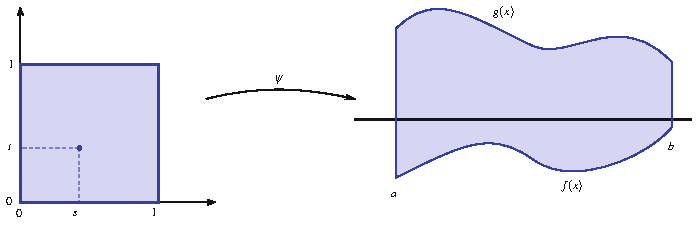
\includegraphics[width=0.960\linewidth]{images/vector/fig-11-30.pdf}
  \caption{几乎任何区域都可以被重新参数化为单位立方体，或被分解成可以重新参数化为单位立方体的若干块}
  \label{fig:11-30}
\end{figure}

\begin{question}\label{q:11-14}
证明 $\psi:I^2\to D$ 是一一且满的.
\end{question}

\begin{question}\label{q:11-15}
证明 $\varphi\circ\psi:I^2\to M$ 是一个由 $I^2$ 参数化的曲面，从而 Stokes 定理的证明适用于 $M$.
\end{question}

对大于二的维数可以作类似的构造. 于是我们论证了 Stokes 定理
\[
\int_M d\alpha=\int_{\partial M}\alpha
\]
适用于任何这样的流形：其参数化可以被重新参数化为单位立方体，或者被分解成随后可以重新参数化为单位立方体的若干块. 不深入技术细节的话，这本质上适用于所有流形.

\section{可视化 Stokes 定理}

在本节中，我们将尝试基于第 5 章的材料，为广义 Stokes 定理的含义提供一幅漫画式的图画，至少在三维情形下如此. 这种讲述方式更接近物理学家有时可视化微分形式的方式，而不是数学家通常采取的观点. 这种可视化技术实际上并不一般，有些流形和形式会使它失效、不起作用；然而，在适用时，它确实提供了一种看待 Stokes 定理的非常优美、几何上直观的方式. 特别是，我们将依赖第 5.5 节发展的可视化. 借助 Stokes 定理，我们将能够对这些可视化获得略微更细致入微的观点，至少在可以进行这些可视化的情形下如此. 在本节中，我们将把这些思想串联起来.

首先我们回顾，在 $\mathbb{R}^3$ 中，我们可以把 1-形式可视化为充满 $\mathbb{R}^3$ 的薄片（如图~\ref{fig:5-36} 所示），把 2-形式可视化为充满 $\mathbb{R}^3$ 的管子（如图~\ref{fig:5-40} 所示），把 3-形式可视化为充满 $\mathbb{R}^3$ 的小立方体（如图~\ref{fig:5-30} 所示）. 我们将一如既往地把 $\mathbb{R}^3$ 上的 0-形式 $f$ 看作函数，即每个点 $p\in\mathbb{R}^3$ 上附着一个值 $f(p)$. 我们还将回顾，若 $d\omega=0$，则微分形式 $\omega$ 称为闭的.

我们将从考虑 0-形式 $f$ 开始. 显然 $df$ 是一个 1-形式，我们可以把它想象成充满空间的薄片. 一维流形是曲线 $C$，所以在 0-形式 $f$ 的情形下，Stokes 定理给出
\[
\int_C df=\int_{\partial C}f.
\]
从第 9.5.2 节我们知道，这当然就是线积分基本定理. 当我们沿 $C$ 移动时，$df$ 的积分计算的是曲线 $C$ 穿过的 1-形式 $df$ 的薄片数. 见图~\ref{fig:11-31}.

\begin{figure}[htbp]
  \centering
  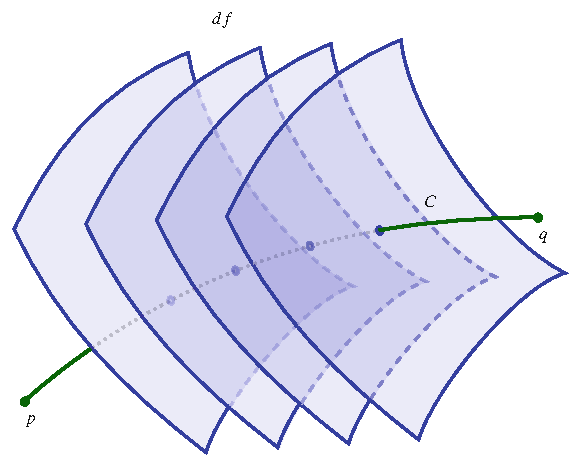
\includegraphics[width=0.689\linewidth]{images/vector/fig-11-31.pdf}
  \caption{一条穿过 $df$ 的薄片的曲线 $C$. 在这幅图中，$\int_C df=4$. 因此，由 Stokes 定理我们知道 $\int_{\partial C}f=f(q)-f(p)=4$. 我们可以把薄片数看作由函数在点 $p$ 与 $q$ 之间的取值变化给出}
  \label{fig:11-31}
\end{figure}

\begin{question}\label{q:11-16}
基于你所知道的关于 1-形式如何写成薄片以及线积分如何计算的知识，论证 $\int_C df$ 确实计算的是曲线 $C$ 穿过的 $df$ 的薄片数.
\end{question}

\begin{question}\label{q:11-17}
假设 $f$ 是闭的，即 $df=0$. 这对函数 $f$ 说明了什么？以图~\ref{fig:11-31} 作为参考.
\end{question}

\begin{question}\label{q:11-18}
基于最后两个问题，我们如何利用 $f$ 来帮助我们画出 1-形式 $df$ 的薄片？
\end{question}

接下来我们考虑 1-形式 $\alpha$. 由于 $\alpha$ 是 1-形式，我们可以把它可视化为充满 $\mathbb{R}^3$ 的薄片，而它的外微分 $d\alpha$ 是 2-形式，可以把它可视化为充满 $\mathbb{R}^3$ 的管子. 这两幅图画究竟如何关联？二维流形是曲面 $S$，其边界是曲线，$\partial S=C$. 我们转向 Stokes 定理
\[
\int_S d\alpha=\int_{\partial S}\alpha.
\]
从第 9.5.3 节我们知道，这当然就是 Stokes 定理的向量微积分版本. $\int_S d\alpha$ 计算的是穿过曲面 $S$ 的 $d\alpha$ 的管子数，而如前所述，$\int_{\partial S}\alpha$ 计算的是 $\alpha$ 的薄片数. 由 Stokes 定理，这两者是相同的. 见图~\ref{fig:11-32}. 基于 Stokes 定理，穿过 $S$ 的 $d\alpha$ 的管子数等于穿过 $\partial S$ 的 $\alpha$ 的薄片数，所以在某种意义上，$d\alpha$ 的每一根管子都会产生额外的 $\alpha$ 薄片.

\begin{figure}[htbp]
  \centering
  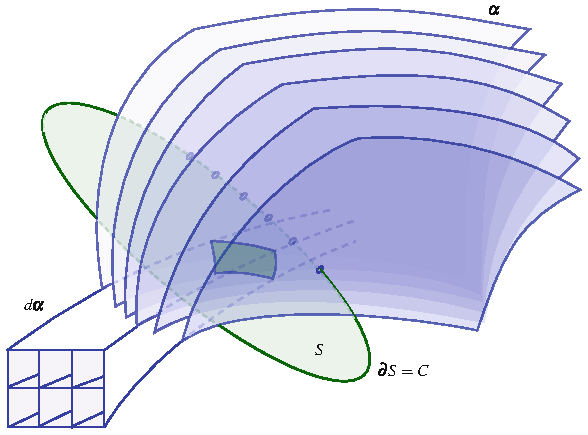
\includegraphics[width=0.696\linewidth]{images/vector/fig-11-32.pdf}
  \caption{带边界 $\partial S=C$ 的曲面 $S$. 在图中，1-形式 $\alpha$ 被描绘成薄片，2-形式 $d\alpha$ 被描绘成管子. 这里 $\int_{\partial S}\alpha$ 计算的是曲线 $C$ 穿过的薄片数，而 $\int_S d\alpha$ 计算的是穿过曲面 $S$ 的管子数. 在这幅图中，$\int_S d\alpha=6$ 且 $\int_{\partial S}\alpha=6$. 我们可以把 $\alpha$ 的薄片想象成从 $d\alpha$ 的管子发出，每根管子对应一片}
  \label{fig:11-32}
\end{figure}

\begin{question}\label{q:11-19}
基于你所知道的关于 2-形式如何描绘成管子以及曲面积分如何计算的知识，论证 $\int_S d\alpha$ 确实计算的是穿过 $S$ 的 $d\alpha$ 的管子数.
\end{question}

\begin{question}\label{q:11-20}
假设 $\alpha$ 是闭的. 这对穿过 $S$ 的管子数或穿过 $\partial S=C$ 的薄片数说明了什么？即使 $d\alpha=0$，$\alpha$ 仍然可能具有薄片吗？画出这种情况的草图.
\end{question}

如果 $\alpha$ 是 2-形式，那么它可以被可视化为充满 $\mathbb{R}^3$ 的管子，而外微分 $d\alpha$ 是 3-形式，可以被可视化为充满 $\mathbb{R}^3$ 的小立方体. 三维流形是体积 $V$，其边界是曲面，$\partial V=S$. Stokes 定理变成
\[
\int_V d\alpha=\int_{\partial V}\alpha.
\]
从第 9.5.4 节我们知道，这当然就是向量微积分中的散度定理. 积分 $\int_V d\alpha$ 计算的是体积 $V$ 内部的 $d\alpha$ 的立方体数，而 $\int_{\partial V}\alpha$ 计算的是穿透曲面 $S$ 的 $\alpha$ 的管子数. 这导致一幅与前面两幅非常相似的图画，见图~\ref{fig:11-33}. 由于根据 Stokes 定理这两者是相等的，我们可以想象 $\alpha$ 的管子从 $d\alpha$ 的立方体发出，每个立方体对应一根管子.

\begin{figure}[htbp]
  \centering
  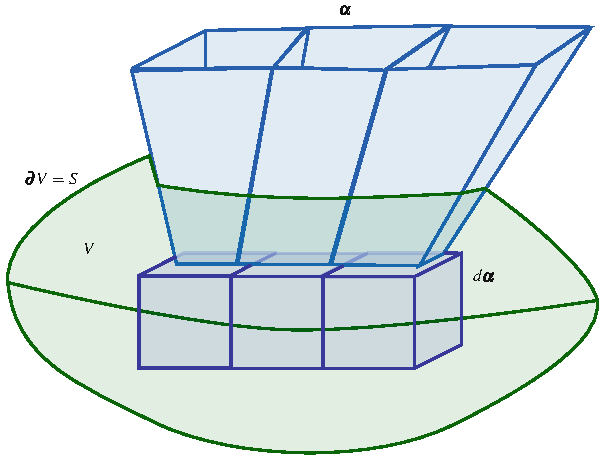
\includegraphics[width=0.717\linewidth]{images/vector/fig-11-33.pdf}
  \caption{带边界 $\partial V=S$ 的体积 $V$. 在图中，2-形式 $\alpha$ 被描绘成管子，3-形式 $d\alpha$ 被描绘成立方体. 这里 $\int_{\partial V}\alpha$ 计算的是穿过曲面 $S$ 的管子数，而 $\int_V d\alpha$ 计算的是包含在体积 $V$ 中的立方体数. 在这幅图中，$\int_V d\alpha=3$ 且 $\int_{\partial V}\alpha=3$. 我们可以把 $\alpha$ 的管子想象成从 $d\alpha$ 的立方体发出，每个立方体对应一根管子}
  \label{fig:11-33}
\end{figure}

\begin{question}\label{q:11-21}
基于你所知道的关于 3-形式如何描绘成立方体以及体积积分如何计算的知识，论证 $\int_V d\alpha$ 确实计算的是 $V$ 内部 $d\alpha$ 的立方体数.
\end{question}

\begin{question}\label{q:11-22}
假设 $\alpha$ 是闭的. 这对 $V$ 内部的立方体数或穿过 $\partial V=S$ 的管子数说明了什么？即使 $d\alpha=0$，仍然可能存在管子吗？画出这种情况的草图.
\end{question}

正如你所记得的，在第 4 章中我们花了很大力气从各种不同的观点引入外微分. 我们这样做是因为外微分在本书以及一般的微分几何和物理学中扮演着基础性的角色. 在第 4.5 节中，我们提供了我们认为的外微分最美好的几何意义之一. 然而，那个观点依赖于对形式积分的理解，而那时我们还没有覆盖积分. 我们现在准备回到那一节所呈现的外微分的几何图画，以便更充分地理解外微分的几何，至少在三维情形下如此. 在那一节中，我们考察了 2-形式 $\omega$，并得到了关于 $d\omega(v_1,v_2,v_3)$ 的如下公式：
\[
\begin{aligned}
d\omega(v_1,v_2,v_3)&=\lim_{h\to 0}\frac{1}{h^3}\int_{\partial(hP)}\omega\\
&=\lim_{h\to 0}\frac{1}{h^3}\Bigl[\int_{hP_{(1,1)}}\omega-\int_{hP_{(1,0)}}\omega-\int_{hP_{(2,1)}}\omega+\int_{hP_{(2,0)}}\omega+\int_{hP_{(3,1)}}\omega-\int_{hP_{(3,0)}}\omega\Bigr]\\
&=\lim_{h\to 0}\frac{1}{h^3}\Bigl[\int_{hP_{(1,1)}}\omega-\int_{hP_{(1,0)}}\omega\Bigr]-\lim_{h\to 0}\frac{1}{h^3}\Bigl[\int_{hP_{(2,1)}}\omega-\int_{hP_{(2,0)}}\omega\Bigr]\\
&\ +\lim_{h\to 0}\frac{1}{h^3}\Bigl[\int_{hP_{(3,1)}}\omega-\int_{hP_{(3,0)}}\omega\Bigr].
\end{aligned}
\]
（分别见图~\ref{fig:11-34} 的左、中、右部分.）

\begin{figure}[htbp]
  \centering
  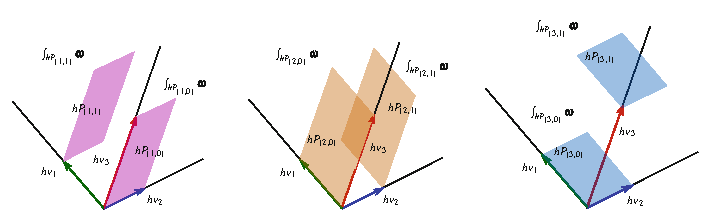
\includegraphics[width=0.960\linewidth]{images/vector/fig-11-34.pdf}
  \caption{出现在积分 $\int_{\partial(hP)}\omega$ 中的立方体 $\partial(hP)$ 的六个面. 积分 $\int_{hP_{(1,1)}}\omega$ 是穿过曲面 $hP_{(1,1)}$ 的管子数. 积分 $\int_{hP_{(1,0)}}\omega$ 是穿过曲面 $hP_{(1,0)}$ 的管子数，依此类推. 这六项按照与面的定向一致的方式相加或相减，得到 $\int_{\partial(hP)}\omega$}
  \label{fig:11-34}
\end{figure}

但现在我们对这在图形上表示什么有了更好的认识. 如果 $\omega$ 是 2-形式，那么我们把它想成充满空间的管子. 积分 $\int_{hP_{(1,1)}}\omega$ 是穿过平行六面体 $hP$ 的 $hP_{(1,1)}$ 面的管子数. 类似地，积分 $\int_{hP_{(1,0)}}\omega$ 是穿过 $hP$ 的 $hP_{(1,0)}$ 面的管子数. 这两个积分之差，就是在 $v_1$ 方向上这两个面之间的管子数之差. 当然，我们必须注意管子的定向才能得到正确的积分符号，但当我们实际计算时，这自然就出来了. 其他方向类似处理. 当我们把各项求和时，我们得到在某一点处、在 $v_1$、$v_2$ 和 $v_3$ 方向上、与平行六面体 $P=\operatorname{span}\{v_1,v_2,v_3\}$ 的边界定向相容的管子数净变化. 见图~\ref{fig:11-34}.

\begin{question}\label{q:11-23}
对 1-形式 $\alpha$ 重复这一分析，以解释外微分 $d\alpha$ 的几何.
\end{question}

\section{小结、参考文献与问题}

\subsection{小结}

Stokes 定理是关于流形上形式积分的主要结果. 它断言：若 $M$ 是光滑的有向 $n$ 维流形，$\alpha$ 是 $M$ 上的 $(n-1)$-形式，则
\[
\int_M d\alpha=\int_{\partial M}\alpha,
\]
其中 $\partial M$ 具有诱导定向.

\subsection{参考文献与进一步阅读}

可能没有任何一本流形理论或微分几何的书籍不覆盖 Stokes 定理，但这里的讲述大体上遵循了 Hubbard 与 Hubbard~\cite{ref27}、Edwards~\cite{ref17} 和 Spivak~\cite{ref40}. 虽然这一讲述试图相当彻底并覆盖大多数情形，但我们选择忽略几层使定理完全一般化的技术细节. 特别是，我们忽略了与带边流形相关的技术细节. 另外，如前所述，也可以不用 $k$-立方体而用 $k$-单纯形的链来证明整个定理，这正是 Flanders~\cite{ref19} 采用的方法. 在可视化 Stokes 定理（至少在三维情形下）方面，我们依赖了第 5 章的材料以及 Warnick、Selfridge 与 Arnold 的论文~\cite{ref49}.

\subsection{问题}

\begin{question}\label{q:11-24}
利用 Stokes 定理求 $\int_C\alpha$，其中 $\alpha=(2xy^3+4x)\,dx+(3x^2y^2-9y^2)\,dy$ 是 $\mathbb{R}^2$ 上的 1-形式，而 $C$ 是从 $(3,2)$ 到 $(5,4)$ 的线段. 然后求 $C$ 为从 $(5,4)$ 到 $(3,2)$ 的线段时的 $\int_C\alpha$.
\end{question}

\begin{question}\label{q:11-25}
利用 Stokes 定理求 $\int_C\alpha$，其中 $\alpha=(6x^2-3y)\,dx+(8y-3x)\,dy$ 是 $\mathbb{R}^2$ 上的 1-形式，而 $C$ 是从 $(3,3)$ 到 $(2,2)$ 的线段. 然后求 $C$ 为从 $(2,2)$ 到 $(3,3)$ 的线段时的 $\int_C\alpha$.
\end{question}

\begin{question}\label{q:11-26}
设 $S$ 是 $\mathbb{R}^2$ 中由 $y=3x$ 和 $y=x^2$ 围成的区域. 选取 $C_1$ 和 $C_2$ 使得 $\partial S=C_1+C_2$. 设 $\alpha=x^2y\,dx+y\,dy$ 是 $\mathbb{R}^2$ 上的 1-形式. 直接求 $\int_S d\alpha$. 然后求 $\int_{\partial S}\alpha$. 验证 Stokes 定理成立.
\end{question}

\begin{question}\label{q:11-27}
设 $S$ 是 $\mathbb{R}^2$ 中第一象限内单位圆的四分之一. 设 $C_1$ 由 $\gamma_1(\theta)=\bigl(\cos(\theta),\sin(\theta)\bigr)$（$0\leq\theta\leq\frac{\pi}{2}$）给出，设 $C_2$ 是从 $(0,1)$ 到 $(0,0)$ 的线段，设 $C_3$ 是从 $(0,0)$ 到 $(1,0)$ 的线段. 因此 $\partial S=C_1+C_2+C_3$. 设 $\alpha=xy\,dx+x^2\,dy$. 利用 Stokes 定理求 $\int_{C_1}\alpha$.
\end{question}

\begin{question}\label{q:11-28}
对 $M$ 为单位圆盘 $x^2+y^2\leq 1$ 且 $\alpha=xy\,dy$，验证 Stokes 定理.
\end{question}

\begin{question}\label{q:11-29}
对 $M=\left\{(u+v,\ u-v^2,\ uv)\,\bigl|\,0\leq u\leq 1,\ 0\leq v\leq 2\right\}$ 且 $\alpha=3z^2\,dx$，验证 Stokes 定理.
\end{question}

\begin{question}\label{q:11-30}
对 $M=\left\{(u^2\cos(v),\ u^3\sin(v),\ u^2)\,\bigl|\,0\leq u\leq 2,\ 0\leq v\leq 2\pi\right\}$ 且 $\alpha=-yz\,dx+xz\,dy$，验证 Stokes 定理.
\end{question}

\begin{question}\label{q:11-31}
设 $V$ 是 $\mathbb{R}^3$ 中的一个体积. 证明 $V$ 的三维体积由下式给出：
\[
\int_{\partial V}\frac{1}{3}\bigl(z\,dx\wedge dy+y\,dz\wedge dx+x\,dy\wedge dz\bigr).
\]
\end{question}

\begin{question}\label{q:11-32}
对 $M$ 为单位立方体 $0\leq x\leq 1,\ 0\leq y\leq 1,\ 0\leq z\leq 1$ 且 $\alpha=2xz\,dx\wedge dy+x\,dy\wedge dz-y^2\,dz\wedge dx$，验证 Stokes 定理.
\end{question}
